
\documentclass[12pt,twoside]{article}

\usepackage{styles/weiiszablon}
\usepackage{styles/listings-rust}
% uzywane do wyrownywania obrazkow (FloatBarrier)
\usepackage{placeins}

\author{Michał Majda}

\studentID{EF-157100}
\title{Proceduralne generowanie map \\ z wykorzystaniem w grze typu roguelike }
\titleEN{Temat pracy po angielsku}
\newcommand{\rodzajPracyNo}{1}
\supervisor{dr hab. inż. Maciej Kusy, prof. PRz }
\supervisorEN{(academic degree) Imię i nazwisko opiekuna}

\abstract{Treść streszczenia po polsku}
\abstractEN{Treść streszczenia po angielsku}

\begin{document}

% strona tytułowa
\maketitle

\blankpage
\tableofcontents
\clearpage
\blankpage


% \section*{Wykaz symboli, oznaczeń i skrótów (opcjonalny)}
% \addcontentsline{toc}{section}{Wykaz symboli, oznaczeń i skrótów (opcjonalny)}%
%
% 1 $\div$ 2 stron wykaz ważniejszych symboli i oznaczeń (jeśli jest potrzebny).
% \clearpage

\section*{Wstęp}
Roguelike to gatunek gier komputerowych posiadający elementy gier fabularnych RPG \cite{book_rpg}, bazujący na dużej losowości rozgrywki \cite{bookroguelike}. Losowość w tych grach W głównej mierze opiera się na losowym rozmieszczeniu przeciwników i przedmiotów oraz losowo generowanych mapach. Inna wążną cechą gier Roguelike jest permadeath -- śmierć gracza oznacza konieczność gry od początku. Klasyczne roguelike-i z racji trudnej rozgrywki nie były popularne, ale w ostatnich latach coraz popularniejsze są gry inspirujące się tym gatunek biorąc z niego tylko wybrane elementy. Z powodu standardowej dla roguelike-ów słabej jakościowo grafiki, oraz map tworzonych proceduralnie to znaczy według algorytmów zamiast ręcznie, gry te są stosunkowo proste w produkcji i nawet współcześnie możliwe do zrealizowania przez jedną lub dwie osoby. Nowsze gry posiadające elementy roguelike najczęściej rezygnują z stanardowego dla starszych tytułów systemu turowego oraz ruchu po kwadratowej siatce na rzecz gry w czasie rzeczywistym i swobodnego ruchu. Czyni to nowych przedstawicieli gatunku roguelike bardziej przystępnymi co przekłada się na wzrost popularności \cite{roguelike_popularity}.

Gatunek ten zapoczątkowany został przez grę Rogue w 1980 roku \cite{rogue_game}, od tej gry wzięła się też nazwa gatunku roguelike - Rogue podobne. Rogue gracz eksploruje podziemia walcząc z przeciwnikami oraz zdobywając coraz lepszy ekwipunek, celem ukończenia gry jest zdobycie amuletu Yendoru znajdującego się w najniższym poziomie. Grafika oparka jest o znaki tekstowe w kodowaniu ASCII \cite{book_ascii}, rozgrywka dzieje się w systemie turowym na kwadratowej siatce.

Mimo iż gatunek roguelike rozwinął się znacznie to wciąż powstają gry wierne klasycznym założeniom gatunku. Przykładem takiej gry jest Caves of Qud z 2015 roku \cite{game_coq}. Gra ta posiada wszystkie cechy klasycznego roguelike-a - turowa rozgrywka, permadeath oraz ruch po kwadratowej siatce, jednak klasyczną grafikę tekstową zastąpiono prostą grafiką typu pixel art \cite{source_pixelart}.

Jednym z najbardziej popularnych przykładów nowoczesnych roguelike-ów jest gra The Binding of Isaac z roku 2011 \cite{game_tboi}. Z gatunku roguelike gra ta zaczerpnęła losowe generowanie map, przedmiotów i przeciwników oraz permadeath. W The Binding of Isaac rozgrywka dzieje się w czasie rzeczywistym a ruch gracza nie jest ograniczony do siatki, dzięki temu gra jest bardziej zręcznościowa i łatwiejsza.\\

Głównym celem pracy jest stworzenie gry z gatunku roguelike z proceduralnei generowanymi mapami, oraz omówienie użytych metod generacji map. \\

Struktura pracy jest następująca: W rozdziale pierwszym dokonano szczegółowej charakterystyki porównawczej innych gier z gatunku roguelike: Rogue, Caves of Qud, The Binding of Isaac. Rozdział drugi opisuje grę roguelike stworzoną na potrzeby niniejszej pracy, w rodziale trzecim zaprezentowano proces tworzenia tej gry oraz omówienie metod proceduralnego generowania map.


\clearpage

\section{Charakterystyka porównawcza gier roguelike}

W niniejszym rodziale szczegółowo omówiono przykłowe gry z gatunku roguelike. Omówione gry to 1: Rogue, 2: Caves of Qud, 3: The Binding of Isaac. Gatunek roguelike od swoich początków nie jest mocno popularnym gatunkiem z powodu trudnej rozgrywki, skomplikowanego sterowania oraz prymitywnej oprawy graficznej. Powstały jednak popularne gry, które zaczerpują z gatunku tylko niektóre elementy, co w niektórych przypadka oznacza płynną, prostszą rozgrywkę z elementami roguelike.

\subsection{Rogue}

Rogue: Exploring the Dungeons of Doom to zaprogramowana w 1980 roku przez Michael-a Toy i Glenn-a Wichman w języku C gra, która zapoczątkowała gatunek Roguelike. Gracz wciela się w postać podróżującą w głąb podziemi osadzonych w fantastycznym, średniowiecznym świecie, w celu odnaleznia amuletu Yendoru. Rogue nie posiada wyboru ani konfiguracji postacji, dlatego każdy gracz rozpoczyna grę tą samą postacią. W trakcie rozgrywki napotkać można wielu przeciwników, a w walce z nimi pomagają znajdowane na poziomach przedmioty i ekwpiunek. Podczas eksploracji glebszych poziomów podziemi gracz napotyka coraz trudniejszych przeciwników, lecz także przedmioty, które znajduje są coraz lepsze. Gra Rogue oparta jest o system turowy, przeciwnicy mogą wykonać ruch dopiero po ruchu gracza. W wyniku tego gra pozwala na dowolnie długie przemyślenie każdego ruchu i taktyczne podejście do walki. Każda mapa przedstawiona jest za pomocą siatki kwadratów, w wyniku czego ruch gracza ograniczony jest do 8 kierunków: góra, dół, lewo, prawo i ukosy. 

Z racji ograniczeń sprzętowych w czasach wydania gry Rogue za reprezentację graficzną odpowiadają litery i znaki ASCII w terminalu. Na rysunku \ref{Rogue:scr1} przedstawiono fragment rozgrywki w grze Rogue. Pomarańczowymi liniami oznaczone są ściany pokojów, zielonymi kropkami podłogi, na szaro oznaczono korytarze. Żólta twarz reprezentuje postać gracza przeciwnicy są oznaczani literami jak hobogoblin oznaczony białą literą 'H' na rysunku.

\FloatBarrier
\begin{figure}[h]
	\centering
	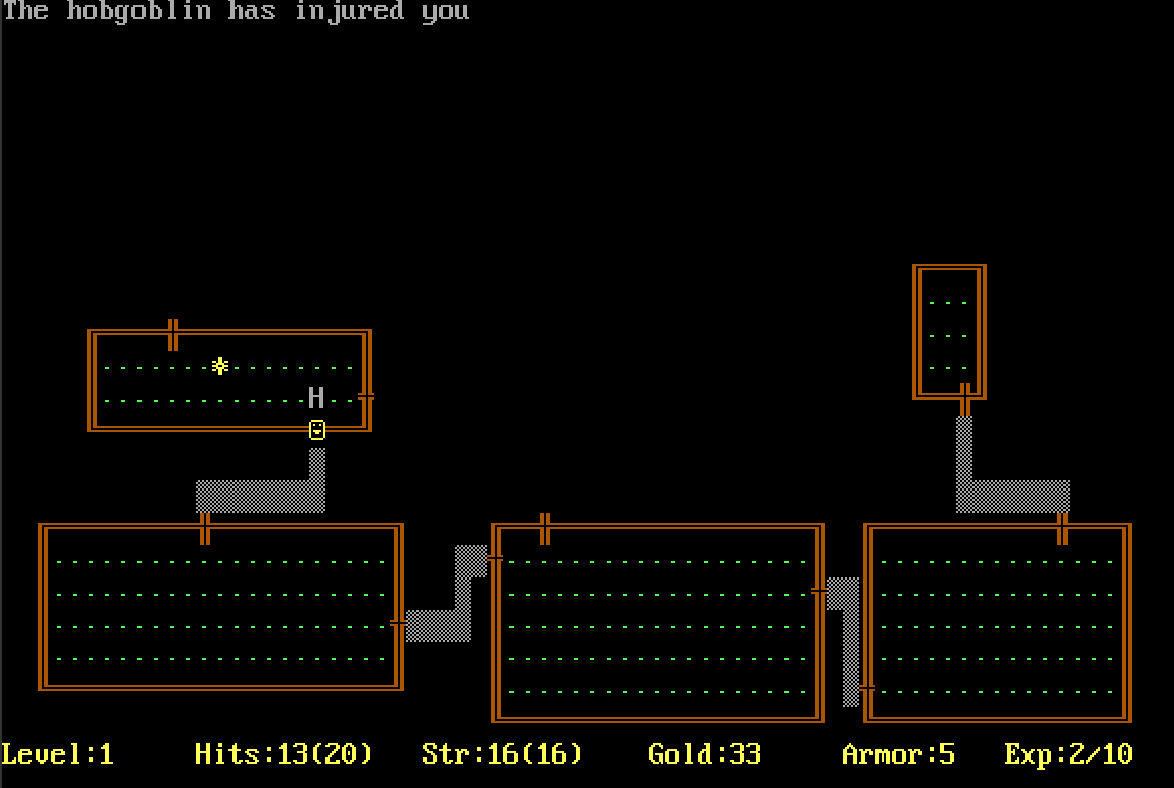
\includegraphics[width=12cm]{images/rogue/scr1.png}
	\caption{Widok główny gry Rogue}
	\label{Rogue:scr1}
\end{figure}
\FloatBarrier

Do sterowania w Rogue używana jest tylko klawiatura, do poruszania przeznaczone są klawisze klawiatury numerycznej a do wykonywania akcji litery -- na przykład klawisz 'I' służy do wyswietlenia ekwipunku. Aby zaatakować gracz musi poruszyć się w stronę przeciwnika będąc tuż przy nim. Wyświetlanie ekwipunku w grze Rogue pokazano na rysunku \ref{Rogue:scr2}, manipulowanie przedmiotami w plecaku nie odbywa się w tym oknie, ale w głownym widoku gry za pomocą odpowienich klawiszy i podania litery odpowiadającej danemu przedmiotowi w ekwipunku. Na przykład aby wyrzucić przedmiot 'a +1, +1 mace` znajdujący się w ekwipunku na rysunku \ref{Rogue:scr2} trzeba wcisnąć klaiwsz 'd' odpowiadający za wyrzucanie przedmiotów i literę 'c' przypisaną obecnie do tego przedmiotu, a w celu zjedzenia 'some food' klaiwsz 'e' odpowiadający za akcję jedzenia i literę 'a'. 

\FloatBarrier
\begin{figure}[h]
	\centering
	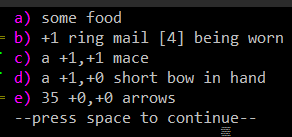
\includegraphics[width=8cm]{images/rogue/scr2.png}
	\caption{Ekran ekwipunku w Rogue}
	\label{Rogue:scr2}
\end{figure}
\FloatBarrier

Rogue zawiera proste proceduralnie generowane mapy, przykładowe dwie mapy pokazano na rysunku: \ref{Rogue:scr3}. Każda mapa zawiera pokoje w układzie siatki 3x3, co szczególnie widać na mapie po prawej na rysunku \ref{Rogue:scr3}, maksymalna liczba pokojów to dziewięć, ale może być ich mniej. Pokoje są połączone ze sobą korytarzami a niektóre przejścia mogą być ukryte przed graczem, co wymusza częste korzystanie z komendy przeszukiwania dostępnej pod klawiszem 'S'. Pokoje i korytarze mogą zawierać ukryte pułapki, które można wykryć używając komendy szukania. Jedyną zmianą w głebszych poziomach są małe labirynty umiejszczone czasami w miejsce niektórych pokojów.

\FloatBarrier
\begin{figure}[h]
	\centering
	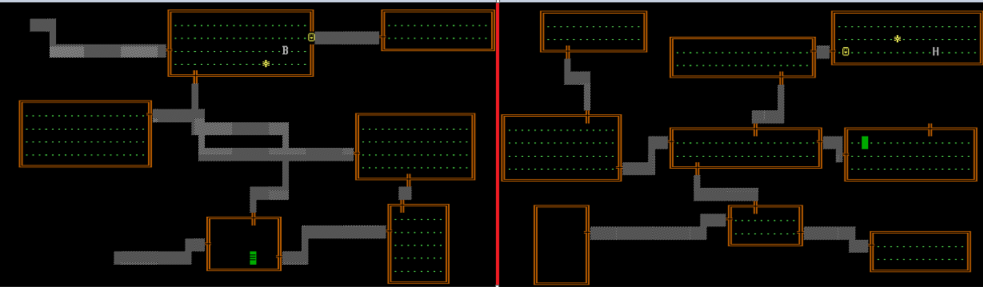
\includegraphics[width=16cm]{images/rogue/scr3.png}
	\caption{Przykładowe mapy w grze Rogue}
	\label{Rogue:scr3}
\end{figure}
\FloatBarrier

Z racji sporego wieku gry Rogue ciężko jest określić jej popularność, jednak z pewnością można stwierdzić, że jest to kluczowa dla gatunku roguelike gra, która stworzyła podwaliny jego głównych cech. Świadczy o tym między innymi sama nazwa gatunku roguelike, która oznacza "podobne do Rogue".



\subsection{Caves of Qud}
Caves of Qud to współczesny przykład rozwoju klasycznej formuły roguelike-ów. Gra tworzona jest w silniku Unity przez studio Freehold Games, wydana została w 2015 roku, lecz rozwijana jest do dzisiaj (stan na luty 2022 roku). Gra posiada wszystkie cechy klasycznego roguelike-a: działa w systemie turowym, posiada permadeath, mapa gry oparta jest o siatkę kwadratów, lecz dodaje też sporo nowoczesnych rozwiązań i znaczne rozwinięcie wielu mechanik gry. Caves of Qud osadzone jest w post apokaliptycznym fantastycznym świecie w którym zaawansowana technologia miesza się z fantastycznymi rasami oraz magią.

Jednym z głównych wyróżników Caves of Qud na tle innych gier tego typu jest bardzo mocno rozwinięty system proceduralnie generowanych map. Gra posiada otwarty świat o statycznie umiejscowionych obszarach takich jak góry, dżungle i pustynie a także miastach, na rysunku \ref{CoQ:scr1} przedstawiono przykładowe mapy wygenerowane w tej grze. Pomimo statycznego ustawienia konkretnych obszarów w grze sam wygląd danych obszarów i miejsc jest proceduralnie generowany, a także na wielu mapach mogą zostać dodane obiekty takie jak ruiny, obozowiska i tym podobne. Główną i najbardziej interesującą metodą uzywaną w tej grze jest generowanie map oparte o Wave Function Collapse (Załamanie funkcji falowej) \cite{coq_wfc}. Metoda ta pozwala na generowanie dowolnych map opartych o mały wzorzec.

\FloatBarrier
\begin{figure}[h]
	\centering
	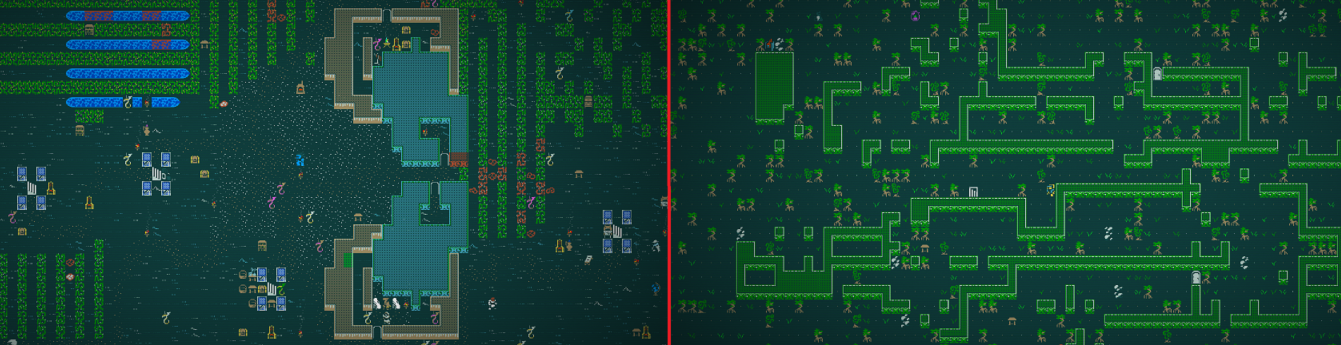
\includegraphics[width=16cm]{images/caves_of_qud/scr1.png}
	\caption{Przykładowe mapy w grze Caves of Qud. Po lewej wioska, po prawej dżungla z ruinami}
	\label{CoQ:scr1}
\end{figure}
\FloatBarrier

Podobnie jak w grze Rogue tutaj również do poruszania się używana jest klawiatura numeryczne i klawisze liter do dostępu do ekwipunku, listy zadań i tym podobne, lecz Caves of Qud umożliwia też granie wyłącznie za pomocą myszki. Gra oferuje bardziej przejrzystę grafikę typu pixel art w formacie 16x24 piksele na jeden kwadrat na mapie, co przedstawiono na rysunku \ref{CoQ:scr3}. Mylącym może być iż gra jest reprezentowana graficznie przez siatkę pionowych prostokątów, lecz w rzeczywistości gra traktuje je jako kwadraty, a ruch w każdym z ośmiu dostępnych kierunków zajmuje w czasie gry tyle samo.

\FloatBarrier
\begin{figure}[h]
	\centering
	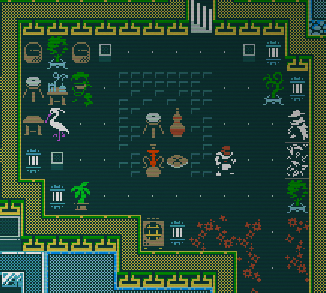
\includegraphics[width=8cm]{images/caves_of_qud/scr3.png}
	\caption{Zrzut ekranu z gry Caves of Qud}
	\label{CoQ:scr3}
\end{figure}
\FloatBarrier

Caves of Qud znacznie rozwinęło też interfejs użytkownika, co znacząco wpływa na ułatwienie rozgrywki. Interfejs jest tu przejrzysty i prosty, dzięki czemu zmiana ekwipunku oraz używanie przedmiotów jest dużo łatwiejsze. Na rysunku \ref{CoQ:scr2} przedstawiono ekran ekwipunku.

\FloatBarrier
\begin{figure}[h]
	\centering
	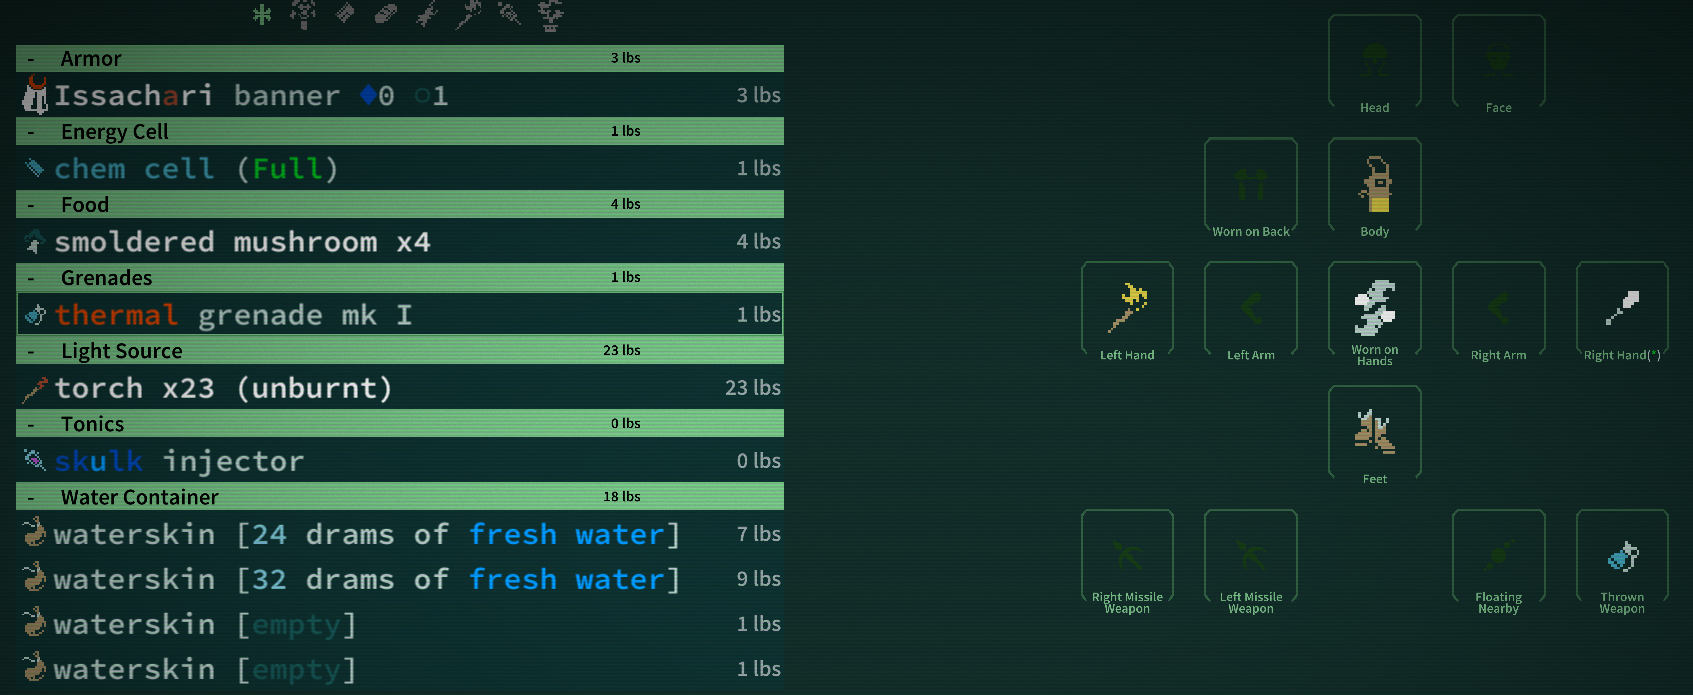
\includegraphics[width=14cm]{images/caves_of_qud/scr2.png}
	\caption{Ekran ekwipunku w Caves of Qud}
	\label{CoQ:scr2}
\end{figure}
\FloatBarrier

Interesującym rozwiązaniem w Caves of Qud jest system handlowy. W grze istnieje system głodu i pragnienia, gracz więc w celu uniknięcia śmierci z głodu lub odwodnienia musi nosić ze sobą zapasy wody i pożywienia, które mają swoją wagę, więc można ich posiadać ograniczoną ilość. Walutą w tej grze jest woda pitna, która jest bardzo rzadko spotykana w postaci źródeł, zdecydowana większość wody w zbiornikach naturalnych jest niezdatna do picia. Z tego powodu gracz zbiera wodę nie tylko dla zaspokojenia pragnienia, ale również w celu handlu z spotykanymi między innymi w wioskach handlarzami. Postać gracza ma ograniczony udźwig, więc często handel sprowadza się do handlu wymiennego, ponieważ trudno jest nosić ze sobą duże kwoty w postaci wody.

Gra Caves of Qud znacznie rozwija aspekt RPG -- odgrywania postaci. W trakcie wyboru postaci najpierw wybiera się typ postaci - mutant mający dostęp do wielu fizycznych lub mentalnych mutacji, które zapewniają dodatkowe zdolności, bonusy lub nawet dodatkowe kończyny lub True Kin będący niezmutowanym człowiekiem, który ma dostęp do cybernetycznych implantów dających różnorodne bonusy i umiejętności. Poza typem wybiera się też pochodzenie postaci, które określa początkowy ekwipunek oraz bonusy do atrybutów. W trakcie gry gracz może dowolnie rozwijać -- zwiększając wartości atrybutów takich jak siła, zręczność, siła woli i tym podobne oraz przez uczenie się nowych umiejętności jak specjizacja w posługiwaniu się konkretnym typem broni lub lepszego unikania ataków. Dzięki dostępowi do dużej ilości różnorodnych mutacji lub implantów, zależnie od typu postaci, gracz dodatkowo może kreować swoją postać na wiele sposobów.

W Caves of Qud proceduralne generowanie używane jest nie tylko do generowania map. W grze można znaleźć duże ilości proceduralnie tworzonych książek, z których część dotyczy także samej fabuły gry \cite{coq_history}. Oznacza to, że poza niektórymi stałymi we wszystkich rozgrywkach aspektami historii również część fabuły będzie inna w każdej nowej rozgrywce.

W odróżnieniu od większości gier tego typu Caves of Qud posiada mocno rozwiniętą historię i rozbudowane główne zadania fabularne. Poza główną linią zadań gra oferuje też sporo losowych zadań, które jednak są dosyć proste i najczęściej sprowadzają się do zdobycia konkretnego przedmiotu lub znalezienia jakiegoś miejsca. Główne zadania są różnorodne, często polegają na odwiedzaniu fabularnych, rozbudowanych lokacji, obronie pewnego miasta przed atakiem lub nawet rozwiązywania zagadek.

Biorąc pod uwagę fakt, że klasyczne gry typu roquelike posiadające dość wysoki poziom trudności rozgrywki, wciąż uznawane są za dość niszowy gatunek. Poszczególne gry zyskują jednak relatywnie dużą popularność, czego przykladem jest Caves Qud, które w serwisie Steam posiada 4356 z czego 95\% jest pozytywnych (stan na luty 2022) \cite{coq_steam}.



\subsection{The Binding of Isaac}

Gra The Binding of Isaac została stworzona w roku 2011 przez Edmund-a McMillen i Florian-a Himsl, a następnie jako remake The Binding of Isaac: Rebirth w roku 2014. W niniejszej pracy skupiono się na omówieniu The Binding of Isaac: Rebirth, gdyż jest to nowsza i bardziej popularna odsłona. Gra ta jest przykładem wzorowania się na roguelike-ach, ale odejściu od części klasycznych założen. Z gatunku zaczerpnięto losowo generowane mapy, losowo rozmieszczane przedmioty i przeciwników, oraz konieczność grania od początku w przypadku śmierci głównej postaci. Rozgrywka w The Binding Isaac dzieje się w czasie rzeczywistym, a ruch postaci nie jest ograniczony do siatki kwadratów. Z tego powodu gra jest bardzo dynamiczna, a walka zręcznościowa.

The Binding of Isaac odeszło od podziału mapy na kwadratową siątke, ale wciąż korzysta z względnie prostej grafiki typu pixel art, co przedstawiono na rysunku: \ref{tboi:scr1}.

\FloatBarrier
\begin{figure}[h]
	\centering
	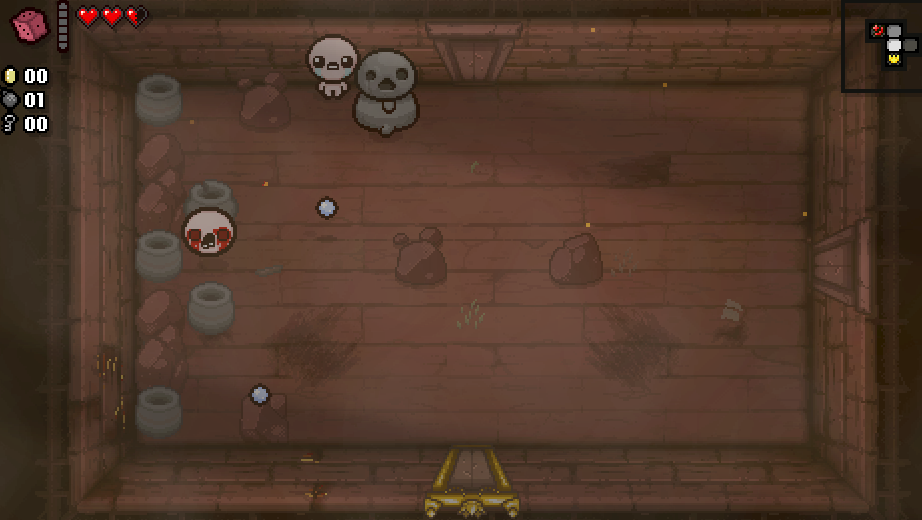
\includegraphics[width=10cm]{images/tboi/scr1.png}
	\caption{Przykład rozgrywki w The Binding of Isaac: Rebirth}
	\label{tboi:scr1}
\end{figure}
\FloatBarrier

Gracz wciela się początkowo w postać Isaac, ale w trakcie rozgrywki może odblokować wiele nowych postaci, które różnią się początkowymi statyskimi takimi jak zdrowie i siła ataku oraz posiadanymi przedmiotami. Gra nie posiada typowego ekwipunku takiego jak zbroje i bronie, zamiast tego w grze zbiera się nieograniczoną ilość przeróżnych przedmiotów, które zapewniają pasywne bonusy. Bonusy te wzmacniają postać na wiele różnych sposobów, od podstawowych zwiększających zdrowie lub atak po takie, które zmieniają łzy, którymi strzela gracz na zupełnie inną postać. Jednym z głównym aututów The Binding of Isaac są możliwe kombinacje przedmiotów, przykładowo jeśli gracz zdobędzie przedmiot, dzięki któremu pociski postaci będą się same nakierowywały na przeciwników, a następnie przedmiot, który zamienia pociski na laser, to ten laser będzie zaginany tak, aby zawsze trafiać przeciwników bez konieczności celowania, co pokazano na rysunku \ref{tboi:scr2}.


\FloatBarrier
\begin{figure}[h]
	\centering
	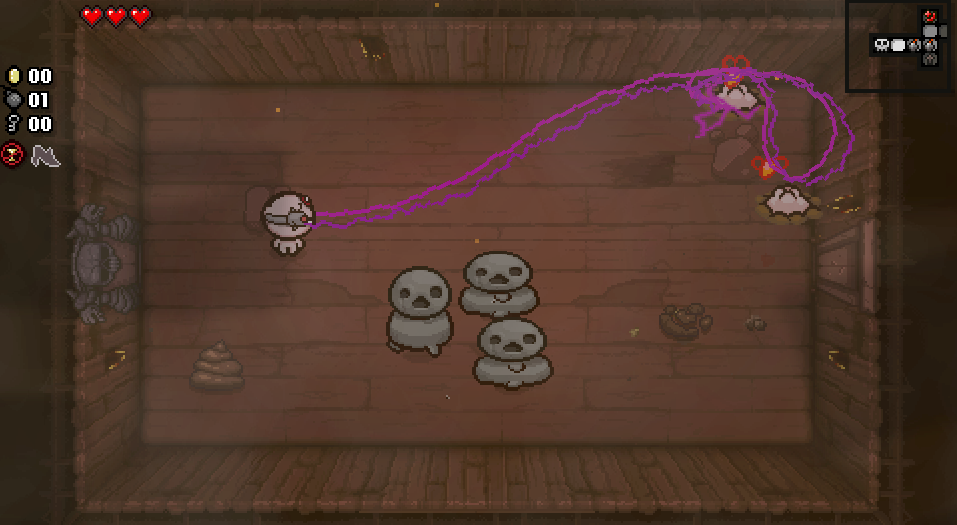
\includegraphics[width=10cm]{images/tboi/scr2.png}
	\caption{Przykład kombinacji przedmiotów w The Binding of Isaac: Rebirth}
	\label{tboi:scr2}
\end{figure}
\FloatBarrier

W grze The Binding of Isaac za sterowanie postacią odpowiadają klawisze 'W', 'A', 'S', 'D' , a za strzelanie klawisze strzałek, do używania przedmiotów jest też używana spacja i klawisz 'Q'. Proste sterowanie jest kolejnym powodem przystępności tej gry.
 W porównaniu do innych gier roguelike losowo generowane mapy w The Binding of Isaac są znacznie prostsze. Gra składa się z wielu poziomów podzielonych na pokoje, każdy z poziomów zakończony jest walką z silnym przeciwnikiem -- bossem. Pokoje są wybierane losowo z puli pokojów przygotowanych przez twórców, a ich rozkład i połączenia są losowo generowane. Na rysunku \ref{tboi:scr3} przedstawiono przykładowy układ poziomów. Z każdym kolejnym poziomem ilość pokojów jest coraz większa, ale jakość napotykanych przedmiotów nie wzrasta. Napotykane przedmioty są kompletnie losowe, dlatego czasem już nawet po pierwszym poziomie postać gracza może posiadać kilka najsilniejszych przedmiotów. 

\FloatBarrier
\begin{figure}[h]
	\centering
	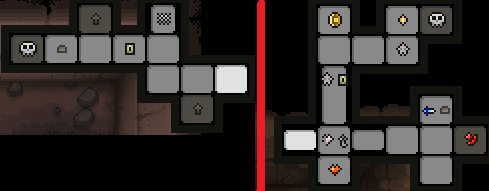
\includegraphics[width=12cm]{images/tboi/scr3.png}
	\caption{Przykładowe układy poziomów w The Binding of Isaac: Rebirth}
	\label{tboi:scr3}
\end{figure}
\FloatBarrier

Jedną z cech gier gatunku roguelike, które implementuje The Binding of Isaac jest permadeath. W porównaniu jednak do innych do tytułów, na których ukończenie trzeba często poświęcić parę godzi, The Binding of Isaac sprawnemu graczowi zajmie około godzinę na ukończenie, w wyniku czego rozpoczynanie rozgrywki od początku nie jest tak dotkliwe, i zachęca do częstego powtórnego przechodzenia gry.


The Binging of Isaac: Rebirth jest jedną z najbardziej popularnych gier z gatunku roguelike, na serwisie Steam posiada 166244 opini, w tym 97\% pozytwnych (stan na luty 2022) \cite{tboi_steam}. Dowodzi to, że przeciętny gracz woli dynamiczną, rozgrywaną w czasie rzeczywistym rozgrywkę od wolnej, taktycznej rozgrywki turowej. Kolejnym dowodem popularności tej gry jest wydana w 2018 roku gra planszowa The Binding of Isaac: Four Souls, która w tydzień zebrała ponad milion dolarów na crowdfundingowym serwisie Kickstarter \cite{tboi_4souls}.



\clearpage	

\section{Szczegółowy opis gry}

W ninejszym rozdziale przedstawiono wszystkie elementy i możliwości gry z gatunku roguelike stworzonej na potrzeby niniejszej pracy.


\subsection{Główne założenia}
Gra stworzona na potrzeby nieniejszej pracy spełnia podstawowe cechy klasycznych gier z gatunku roguelike:

\begin{itemize}
	\item oparta jest o system turowy,
	\item zawiera plansze generowane proceduralnie,
	\item rozmieszczenie przeciwników i przedmiotów jest losowe,
	\item mapy są w postaci siatki kwadratów, ruch postaci oraniczony jest do poruszania się po nich,
	\item postać gracza posiada ekwipunek, który może założyć -- zbroje i bronie,
	\item gra posiada przedmioty, które można użyć -- mikstury i magiczne zwoje,
	\item permadeath - śmierć kończy rozgrwkę, brak możliwości zapisu i wczytania stanu rozgrywki.		
\end{itemize}

Projekt gry posiada też kilka bardziej nowoczesnych aspektów:
\begin{itemize}
	\item grafika typu pixel art,
	\item rozwinięty, prostszy w użytkowaniu interfejs,			
	\item system prezentowania z krokami proceduralnego generowania map.
\end{itemize}

Gra składa się z sześciu różnorodnych, proceduralnie generowanych poziomów, gracz napotyka coraz trudniejszych przeciwników w kolejnych poziomach, a także znajduje coraz lepszy ekwipunek i przedmioty. Celem gry jest pokonanie ostatniego przeciwnika "Mighty Blop", znajdującego się w ostatnim poziomie. Często takiego ostatniego, najsilniejszego przeciwnika określa się w grach jako "Boss". Aby przejść grę gracz powinien eksplorować kolejne poziomy w celu odnalezienia coraz silniejszych przedmiotów i ekwipunku, które niezbędne są przy walce z trudniejszymi przeciwnikami.  Gra osadzona jest w fantastycznym, średniowiecznym świecie, w którym spotkać można rycerzy, gobliny i orków, a także magiczne mikstury i zwoje.


\subsection{Opis menu głównego gry}
Po uruchomieniu gry pierwsze co zobaczy gracz to główne menu przedstawione na rysunku \ref{mygame:scr1}. Menu składa się z żółtego tytułu gry, oraz czterech opcji. Poruszać się po menu można za pomocą klawiszy strzałek, aktualnie wybrana opcja jest zaznaczona na zielono, a wybór opcji przeprowadzany jest klawiszem enter.

\FloatBarrier
\begin{figure}[h]
	\centering
	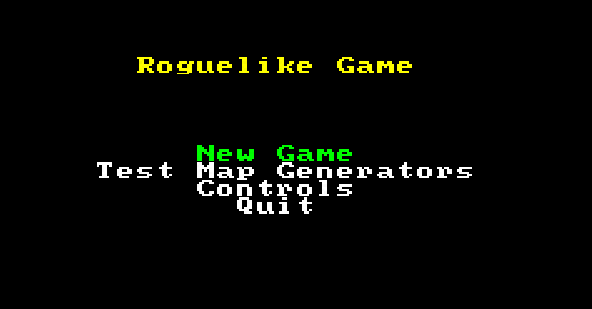
\includegraphics[width=10cm]{images/mygame/scr1.png}
	\caption{Menu główne gry}
	\label{mygame:scr1}
\end{figure}
\FloatBarrier

Menu składa się z następujących opcji:
\begin{itemize}
	\item 'New Game' -- rozpoczęcie nowej gry,
	\item 'Test Map Generators' -- otwiera menu testera proceduralnego generowania map,			
	\item 'Controls' -- otwiera listę komend dostępnych w grze,
	\item 'Quit' -- zamknięcie programu.
\end{itemize}


\subsection{Sterowanie w grze}
 Główną metodą poruszania się postacią jest klawiatura numeryczna, co używane jest od dawna w gatunku roguelike. Jest to także najwygodniejsza kombinacja klawiszy przy możliwości ruchu w ośmiu kierunkach -- dół, gór, prawo, lewo oraz skosy, schemat poruszania się przy użyciu klawiatury numerycznej przedstawiono na rysunku \ref{numpad_controls}. Nie wszystkie klawiatury, a szczególnie te w laptopach, posiadają klawiaturę numeryczną, dlatego gra posiada też alternatywne sterowanie oparte o klawisze strzałek i klawisze liter. Klaiwsz '5' w przypadku klawiatury numerycznej używany jest do pomijania tury, co jest istotną możliwością w grze turowej. Jednokrotne naciśnięcie klaiwsza odpowiadającego za ruch w danym kierunku porusza postać gracza o jedno pole w danym kierunku, jeżeli nie jest ono zajmowane przez ścianę. Jeśli pole na które porusza się gracz zajmowane jest przez przeciwnika, to zamiast ruchu postać gracza wykona atak przeciwko temu przeciwnikowi, jest to standardowa metoda ataku w tego typu grach.
 
\FloatBarrier
\begin{figure}[h]
	\centering
	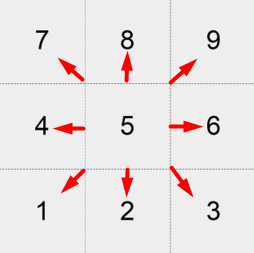
\includegraphics[width=4cm]{images/custom/numpad_controls.png}
	\caption{Schemat sterowania na klawiaturze numerycznej}
	\label{numpad_controls}
\end{figure}
\FloatBarrier

Objaśnienia sterowania i lista dostępnych akcji w grze z menu głównego za pomocą opcji 'Controls' na rysunku \ref{mygame:scr2} przedstawiono widok dostępny po wybraniu tej opcji.

\FloatBarrier
\begin{figure}[h]
	\centering
	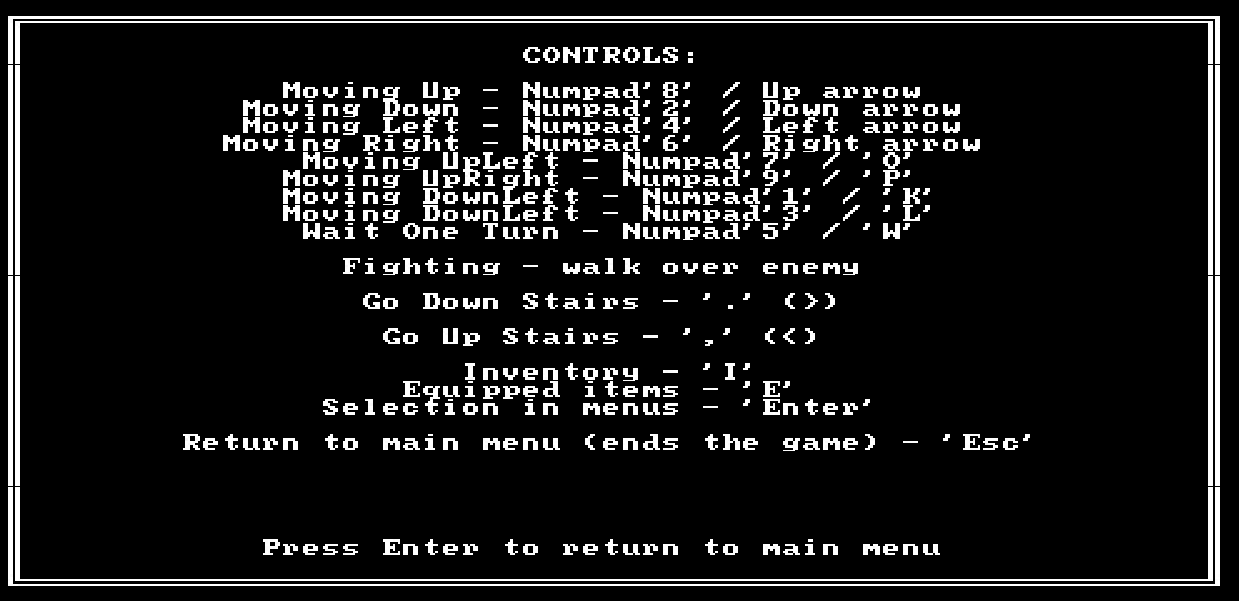
\includegraphics[width=16cm]{images/mygame/scr2.png}
	\caption{Objaśnienia sterowania w grze}
	\label{mygame:scr2}
\end{figure}
\FloatBarrier


Poniżej wyjaśnienie wszystkich komend dostępnych w grze w kolejności z rysunku \ref{mygame:scr2}, Oznaczenie NumpadX oznacza klawisz cyfry X z klawiatury numerycznej. Oznaczenie 'X' oznacza klawisz litery lub znaku X:

\begin{enumerate}
	\item Numpad8 / klawisz strzałki w górę -- poruszenie się w górę,
	\item Numpad2 / klawisz strzałki w dół -- poruszenie się w dół,
	\item Numpad4 / klawisz strzałki w lewo -- poruszenie się w lewo,
	\item Numpad6 / klawisz strzałki w prawo -- poruszenie się w prawo,
	\item Numpad7 / 'O' -- poruszenie się na ukos -- góra, lewo,
	\item Numpad9 / 'P' -- poruszenie się na ukos -- góra, prawo,
	\item Numpad1 / 'K' -- poruszenie się na ukos -- dół, lewo,
	\item Numpad3 / 'L' -- poruszenie się na ukos -- dół, prawo,
	\item Numpad5 / 'W' -- pominięcie jednej tury,
	\item ',' (klawisz przecinka) -- zejście w dół po schodach,
	\item '.' (klawisz kropki) -- wejście w górę po schodach,
	\item 'G' -- podniesienie przedmiotu,
	\item 'I' -- otwarcie menu ekwipunku,
	\item 'E' -- pokazuje obecnie wyekwipowane przedmioty,
	\item klaiwsz Enter -- wybór opcji w menu,
	\item klaiwsz Esc -- powrót do menu głównego, kończy to obecną rozgrywkę,
	\item klawiszem Enter powrócić można z menu `Controls` do menu głównego.
\end{enumerate}


\subsection{Opis poziomów}
Gra składa się z sześciu poziomów oferujących róznych przeciwników i przedmioty. W tej sekcji w celu prezentacji wyglądu poszczególnych poziomów posłużono się testerem proceduralnie generowanych map. Poziomy zaprezentowano w kolejności w jakiej występują one w trakcie rozgrywki. Mapy na poziomach 1-5 są proceduralnie generowane, więc przy każdej nowej rozgrywce ich wygląd będzie podobny, ale odmienny. Również rozmieszczenie przeciwników i przedmiotów na poziomach jest za każdym razem losowe. Akcja gry ma miejsce w podziemnych lochach połączonych z jaskiniami, kolejne poziomy są coraz głębiej w ziemie, dlatego są połączone ze sobą schodami. Gracz ma możliwość swobodnego wracania do poprzednich poziomów.

\subsubsection{Poziom 1}
Poziom pierwszy to kilka prostych pokojów połączonych ze sobą korytarzami, przykładowy układ tej mapy przedstawiono na rysunku \ref{mygame:map1}. Na poziomie tym napotkać można najprostszych przeciwników: 'blip' oraz 'goblin'. Istnieje też mała szansa, że w pokoju z golbinami pojawi się też trudniejszy przeciwnik -- 'orc'. Na poziomie tym znaleźć można podstawowy pancerz i miecz, a także mikstury uzdrawiające i zwoje uśpienia, które są szczególnie przydatne w walkach z trudniejszymi przeciwnikami w późniejszych poziomach.

\FloatBarrier
\begin{figure}[h]
	\centering
	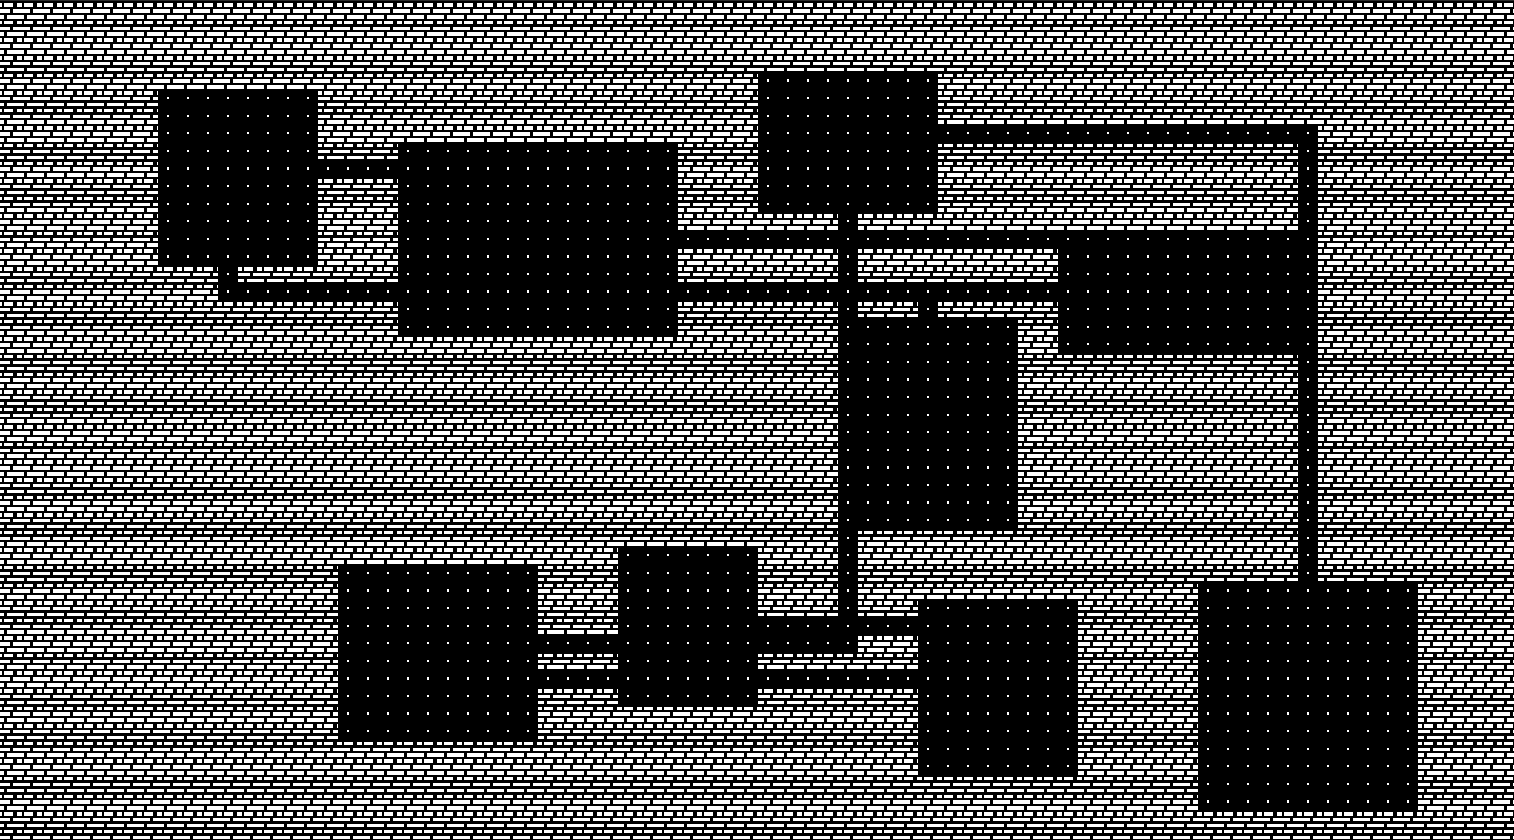
\includegraphics[width=12cm]{images/mygame/map1.png}
	\caption{Przykładowy układ poziomu pierwszego}
	\label{mygame:map1}
\end{figure}
\FloatBarrier


\subsubsection{Poziom 2}
Poziom drugi to bardziej rozwinięta wersja poziomu pierwszego z większą liczbą pokojów i inna metodą generacji. Przykładowy poziom drugi przedstawiono na rysunku \ref{mygame:map2}. Na drugim poziomie spotkać można gobliny z poprzedniego poziomu a także trudniejszych przeciwników 'orc' -- ork oraz 'knight' -- rycerz. Szczególnie trudnym przeciwnikiem na tym poziomie jest rycerz, który wyekwipowany jest w mocną zbroję i miecz, które można zdobyć po jego pokonaniu. W pokoju z rycerzem jest też szansa na znalezienie poteżniejszych magicznych zwojów - zwoju kuli ognia, oraz zwoju teleportacji. Na poziomie tym można też znaleźć małe ilości mocniejszych mikstur uzdrowienia, oraz zwoje magicznych pocisków.


\FloatBarrier
\begin{figure}[h]
	\centering
	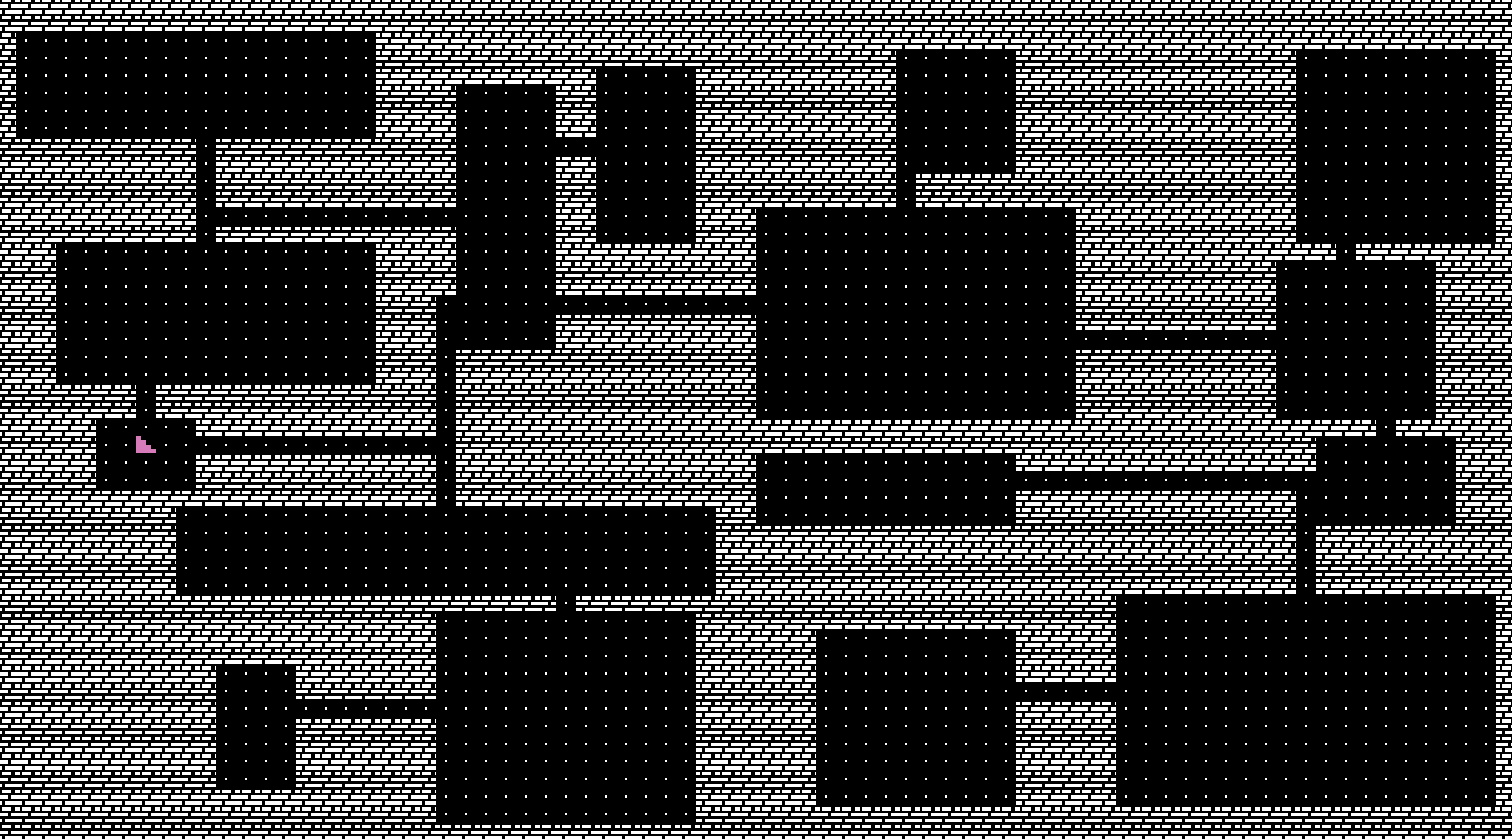
\includegraphics[width=12cm]{images/mygame/map2.png}
	\caption{Przykładowy układ poziomu drugiego}
	\label{mygame:map2}
\end{figure}
\FloatBarrier


\subsubsection{Poziom 3}
Poziom trzeci to duża jaskinia wypełniona masą goblinów i orków. Przykładowy poziom trzeci przedstawiono na rysunku \ref{mygame:map3}. Mimo, że nie spotyka tu się trudniejszych przeciwników niż orkowie, to trudnością tego etapu jest duża liczba przeciwników, oraz duży otwarty teren. Taki układ mapy w przeciwieństwie do ciasnych korytarzy poprzednich poziomów może łatwo doprowadzić do otoczenia gracza przez wielu przeciwników.

\FloatBarrier
\begin{figure}[h]
	\centering
	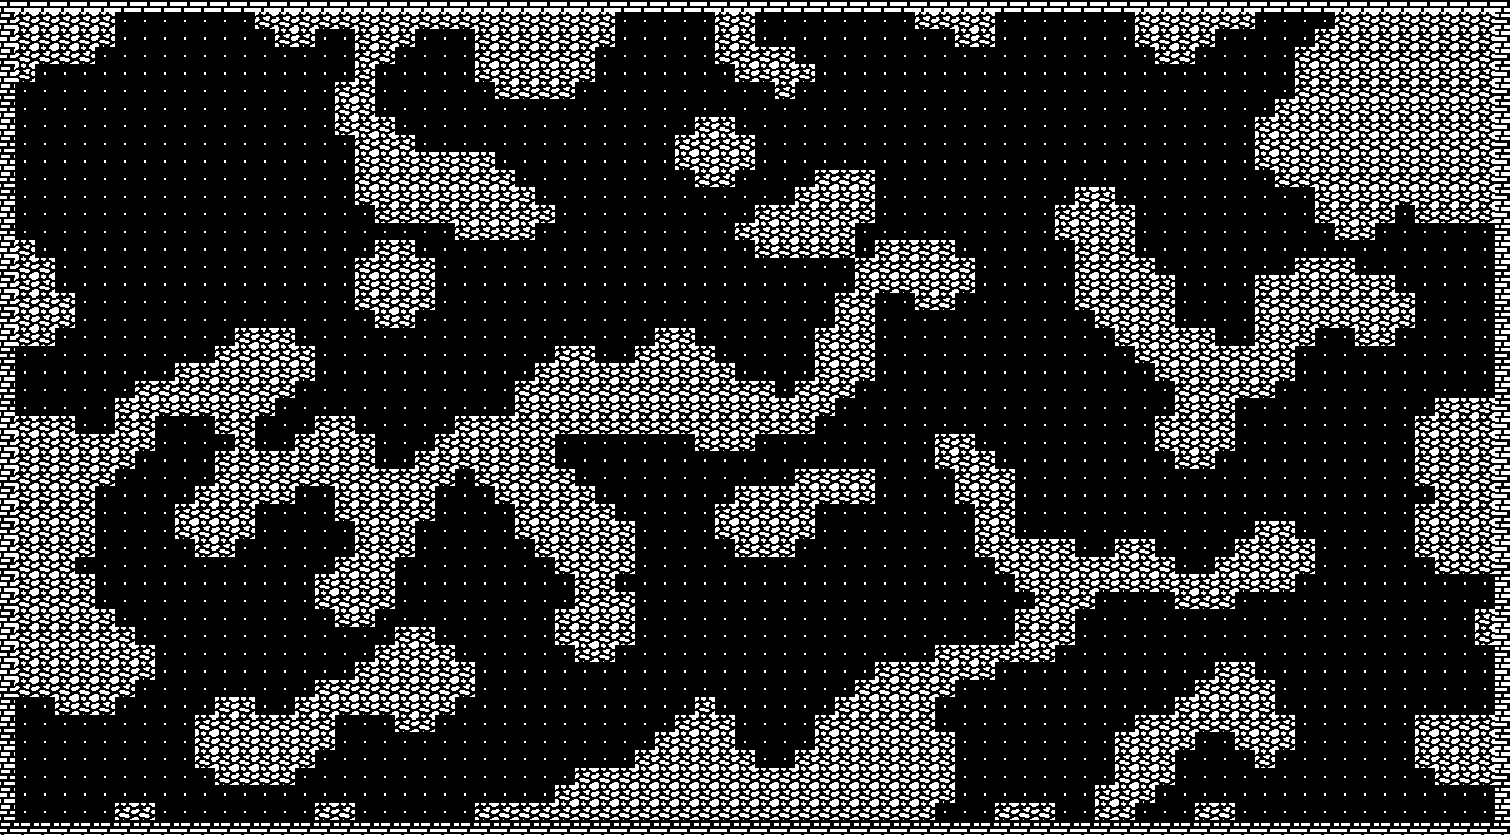
\includegraphics[width=12cm]{images/mygame/map3.png}
	\caption{Przykładowy układ poziomu trzeciego}
	\label{mygame:map3}
\end{figure}
\FloatBarrier


\subsubsection{Poziom 4}
Poziom czwarty to kolejna jaskinia, tym razem z dużo większym obszarem w centrum, oraz okazjonalnymi ciasnymi odnogami. Przykładowy poziom czwarty przedstawiono na rysunku \ref{mygame:map4}. Na poziomie tym można spotkać duże ilości prostych 'blip'ów z pierwszego poziomu, a także sporo ich większych odmian -- 'blop'-ów. 'Blop' poza byciem silniejszą odmianą blipa posiada też specjalną zdolność -- po śmierci rozpadnie się na kilka blipów. Na tym poziomie można też znaleźć mocniejszą zbroję i miecz, a także duże mikstury uzdrowienia i zwoje obszarowego uśpienia.

\FloatBarrier
\begin{figure}[h]
	\centering
	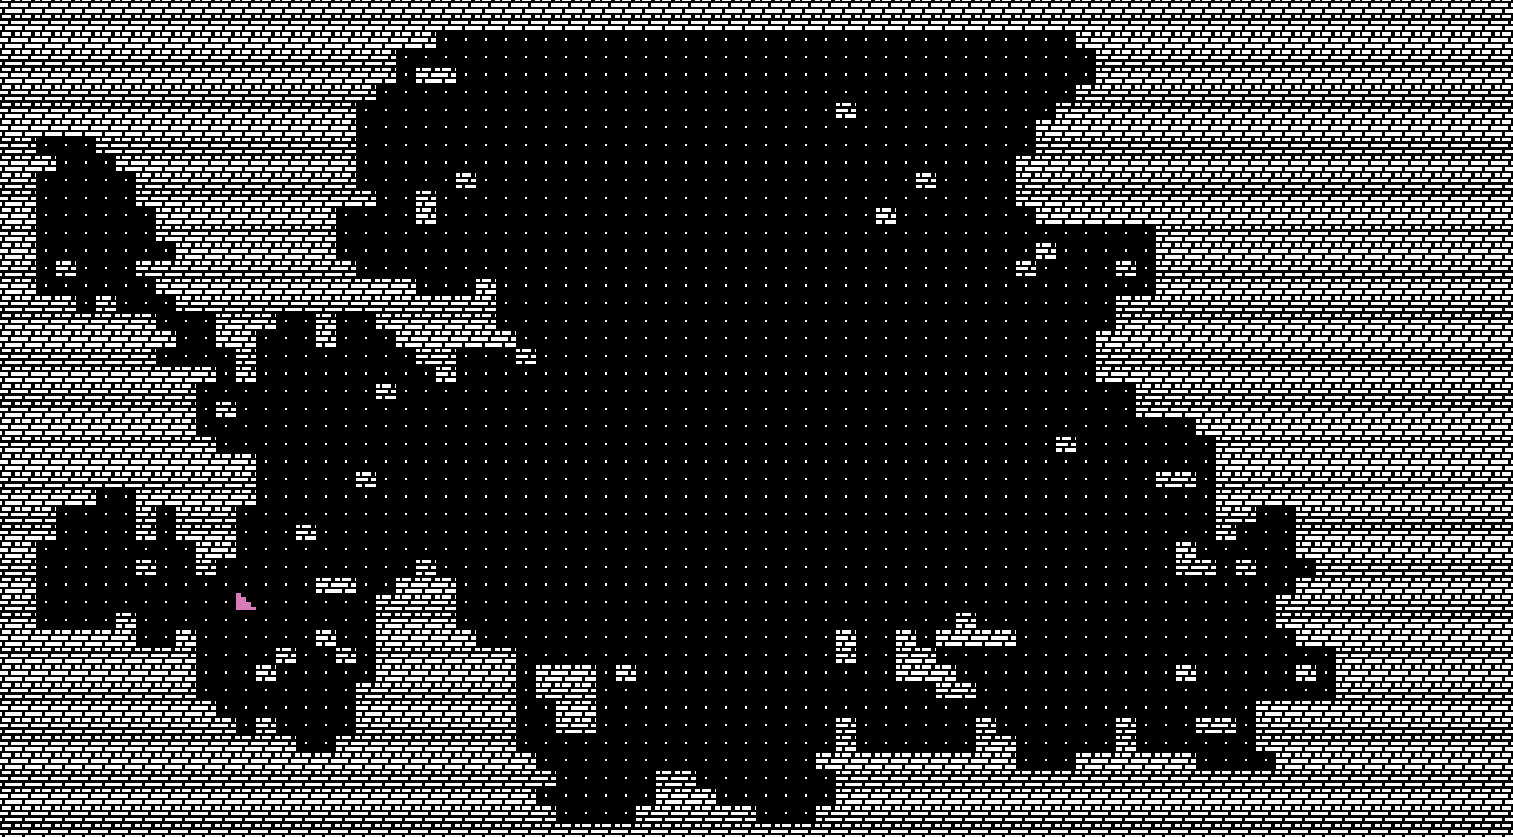
\includegraphics[width=12cm]{images/mygame/map4.png}
	\caption{Przykładowy układ poziomu czwartego}
	\label{mygame:map4}
\end{figure}
\FloatBarrier

\subsubsection{Poziom 5}
Poziom piąty to duży obszar podzielony na pokoje bezpośrednio połączone ze sobą, bez korytarzy. Przykładowy poziom piąty przedstawiono na rysunku \ref{mygame:map5}. Na tym poziomie spotkać można najmocniejszych przeciwników: rycerzy ('knight') oraz łotrzyków ('rogue'). W trakcie eksploracji poziomu piąego odnaleźć można namocniejszą w grze zbroję oraz miecz, co będzie dla gracza szczególnie przydatne na poziomie szóstym.

\FloatBarrier
\begin{figure}[h]
	\centering
	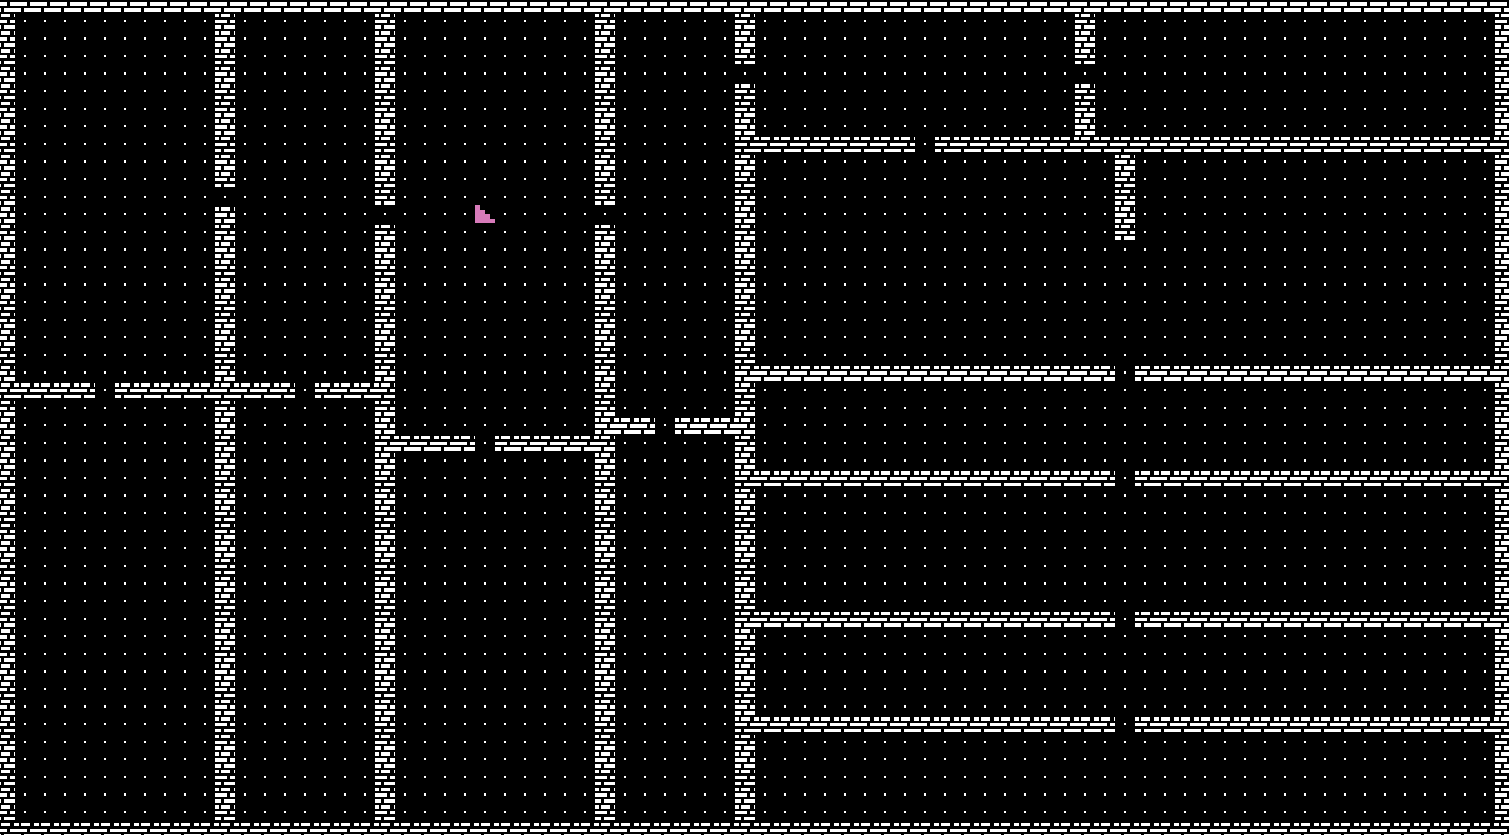
\includegraphics[width=12cm]{images/mygame/map5.png}
	\caption{Przykładowy układ poziomu piątego}
	\label{mygame:map5}
\end{figure}
\FloatBarrier


\subsubsection{Poziom 6}
Poziom szósty to ostatni poziom, cały będący otwartą przestrzenią. W tym poziomie gracz spotka tylko jednego przeciwnika -- 'Mighty Blop' (potężny blop), którego pokonanie jest celem gry. Potężny blop jest silniejszą wariacją blopa, na które rozpada się po śmierci, one z kolei po śmierci rozpadną się na blipy. Aby ukończyć grę należy go pokonać oraz zejść schodami w dół.


\subsection{Okno gry}
Po rozpoczęciu nowej gry gracz zobaczy okno z wycinkiem mapy wycentrowanym na postać gracza, a także okno dziennika zdarzeń i pasek punktów życia, co pokazano na rysunku \ref{mygame:game_window}. Widok mapy jest powiększonym wycinkiem poziomu, przesuwającym się razem z graczem. Na mapie poza ścianami zaznazone są też pola podłogi za pomocą białej kropki. Jest to przydatne w grach opierającch się o ruch na siatce kwadratów do przeliczania odległości. W dzienniku zdarzeń zapisywane są wydarzenia z gry takie jak podnoszenie przedmiotu i ataki gracza lub przeciwników. Pasek życia posiada liczbową prezentację punktów życia w postaci [aktualne punkty zdrowia / maksymalne punkty zdrowia], oraz graficzną reprezentację -- czerwony pasek zmniejszający się wraz ze spadkiem zdrowia. Gracz posiada pole widzenia o określonym zasięgu, któro działa w sposób realistyczny to znaczy będąc blisko wejścia do pokoju jest on w stanie zobaczyć tylko jego skrawek, a nie cały pokój, co widać na rysunku \ref{mygame:game_window}. Poza aktualnie widzianymi polami postać gracza pamięta też obszary, które wcześniej zobaczyła, są one zaznaczone na szaro. Na obszarach, które gracz pamięta, ale nie widzi ich obecnie zaobserwować można tylko układ podłóg i ścian, przeciwników i przedmioty zauważyć można tylko w bezpośrednim polu widzenia.

\FloatBarrier
\begin{figure}[h]
	\centering
	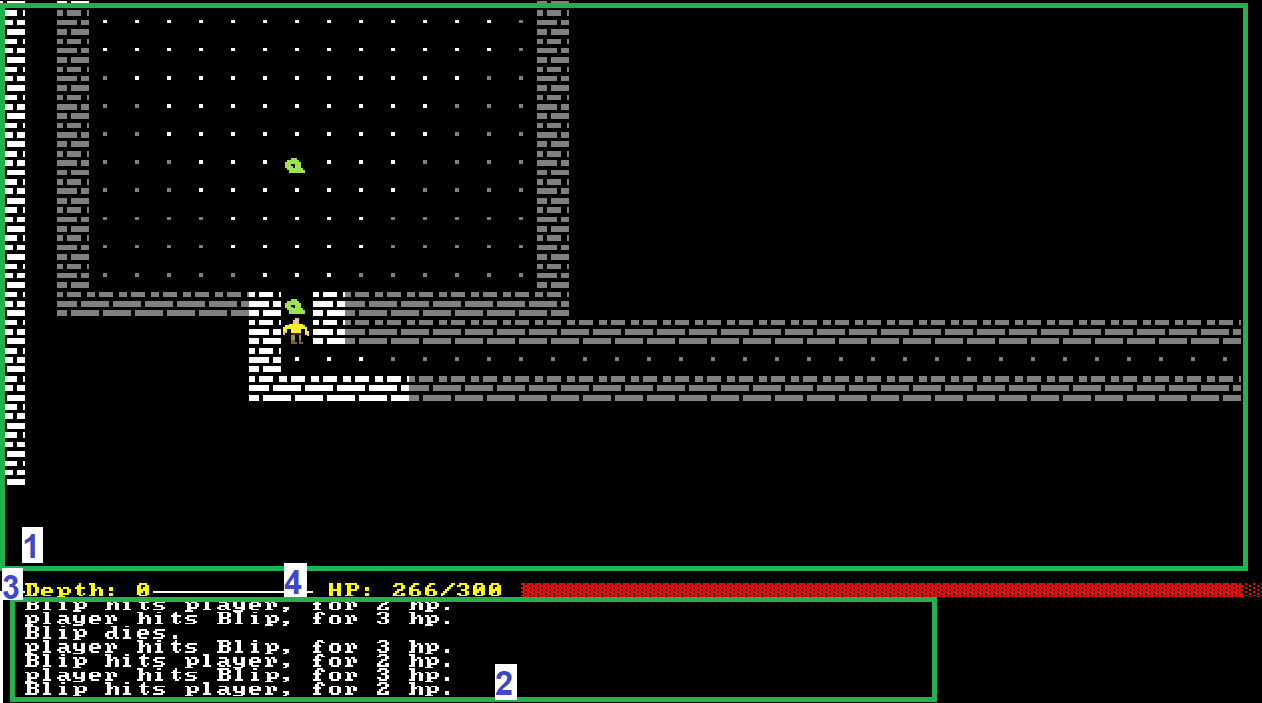
\includegraphics[width=16cm]{images/mygame/game_window.png}
	\caption{Widok główny gry. 1 - aktualny wycinek mapy, 2 - dziennik zdarzeń, 3 - aktualny poziom, 4 - pasek zdrowia. Żółta postać to gracz, a zielone postacie to gobliny -- jeden z typów przeciwników }
	\label{mygame:game_window}
\end{figure}
\FloatBarrier


\subsection{Przedmioty oraz ich używanie}
W grze gracz przez eksplorację znaleźć moze wiele różnorodnych przedmiotów, których używanie jest konieczne w celu ukończenia gry. Przedmioty dzielą się na zbroje, bronie, mikstury oraz magiczne zwoje. Aby podnieść przedmiot gracz musi przejść na zajmowane przez przedmiot pole a następnie wcisnąć klawisz 'G'. Na rysunku \ref{mygame:item_room} przedstawiono pokój wypełniony przedmiotami.

\FloatBarrier
\begin{figure}[h]
	\centering
	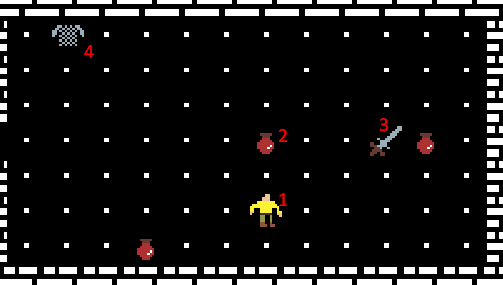
\includegraphics[width=9cm]{images/mygame/item_room.png}
	\caption{Pokój z przedmiotami. 1 - postać gracza, 2 - mikstura zdrowia, 3 - broń, 4 - zbroja }
	\label{mygame:item_room}
\end{figure}
\FloatBarrier


\subsubsection{Okna ekwipunku}
Gracz w każdej chwili może sprawdzić swój ekwipunek klawiszem 'I', ekran ten zaprezentowano na rysunku \ref{mygame:inv}. Wyboru przedmiotu dokonuje się za pomocą stzałek i klawisza Enter, litera po lewej stronie przy aktualnie wybranym przedmiocie jest zaznaczona na zielono. Innym sposobem wybrania przedmiotu jest wciśnięcie przypisanej mu po lewej stronie litery w nawiasach. Dopis '<EQUIPPED>' po prawej stronie danego przedmiotu oznacza, że jest on aktualnie założony przez postać gracza. Zielone liczby oznaczają ilość danego przedmiotu, na rysunku \ref{mygame:inv} zaobserwować można, że gracz posiada cztery mikstury uzdrawiająca 'Health potion'. Klawiszem Esc można wyjśc z menu ekwipunku i powrócić do gry.

\FloatBarrier
\begin{figure}[h]
	\centering
	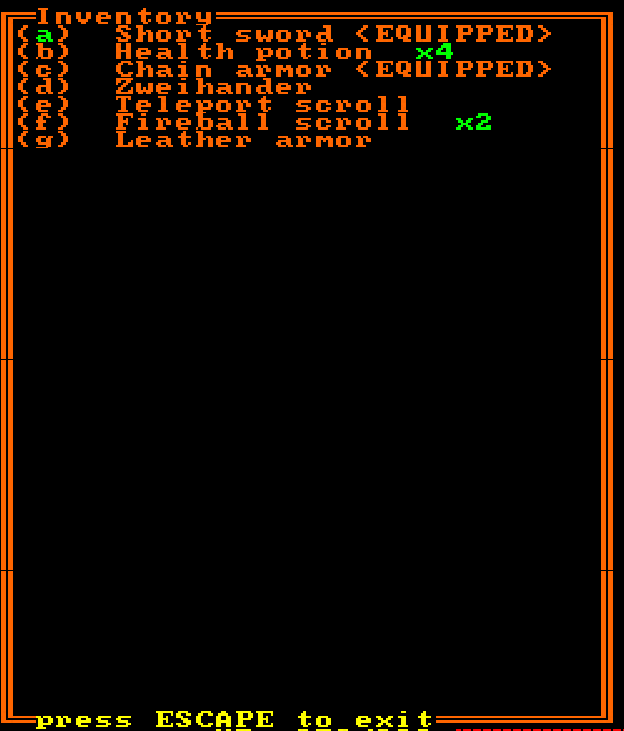
\includegraphics[width=8cm]{images/mygame/inv.png}
	\caption{Okno ekwipunku}
	\label{mygame:inv}
\end{figure}
\FloatBarrier

Po wybraniu przedmiotu wyświetla się menu wyboru akcji dostepnych dla każdego przedmiotu, przykładowe dostępne akcje dla 'Health potion' przedstawiono na rysunku \ref{mygame_item_menu}. Każdy przedmiot można wyrzucić za pomocą akcji 'drop', spowoduje to wyrzucenie przedmiotu na pole zajmowane przez gracza. W przypadku nie założonych zbroi i broni dostępna jest opcja 'Equip' powodująca wyekwipowanie danego przedmiotu. Konsekwentnie założone przedmioty posiadają akcję 'UnEquip', która pozwala na ściągnięcie danego przedmiotu. Mikstury i zwoje posiadają akcję 'Use' pozwalająca na użycie danego przedmiotu. Niektóre przedmioty są używane od razu na postaci gracza, a niektóre pozwalają na wybranie celu.

\FloatBarrier
\begin{figure}[h]
	\centering
	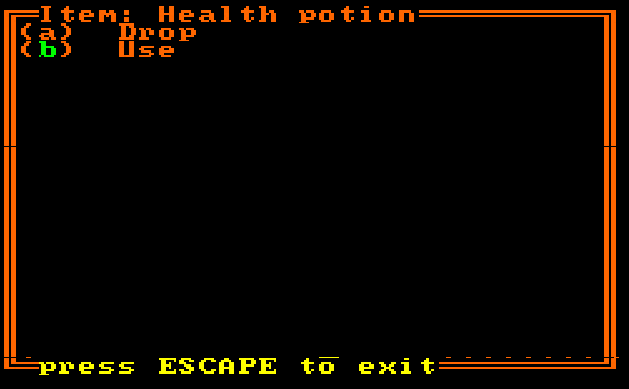
\includegraphics[width=8cm]{images/mygame/item_menu.png}
	\caption{Okno akcji przedmiotu z ekwipunku}
	\label{mygame:item_menu}
\end{figure}
\FloatBarrier


\subsubsection{Zbroje i bronie}
Każda postać w grze posiada wartość obrony, która obniża wartość otrzymywanych obrażeń. Obronę zwiększyć można za pomocą zbroi zakładanych na poszczególne części ciała: głowę, tors, ręce oraz nogi. W grze w kolejnych poziomach spotkać można coraz lepsze zbroje, dzięki czemu postać gracza jest coraz wytrzymalsza.

Podobnie jak obronę, postać gracza oraz przeciwnicy posiadają wartośc ataku, która określa ilość zadawanych w trakcie ataku obrażeń. Wartość tę można zwiększyć ekwipując bronie rozsiane po poziomach. Lepsze bronie znaleźć można w późniejszych poziomach, dzięki czemu gracz, który dokładnie eksploruje plansze będzie zadawał coraz więcej obrażeń. Reprezentację graficzną zbrój oraz broni zaobserwować można na rysunku \ref{mygame:item_room}.


\subsubsection{Mikstury}
Postać gracza posiada określoną ilość punktów zdrowia 'HP', które zmniejszają się wskutek ataków przeciwników. Aby zregenerować zdrowie gracz musi znaleźć mikstury uzdrawiające. W grze dostępne są dwie wersje tych mikstur -- zwykła 'Health potion' oraz większa 'Great health potion', któa leczy większą ilość punktów zdrowia. Użycie mikstur jest natychmiastowe, a celem zawsze jest postać gracza. Wygląd mikstur został pokazany na rysunku \ref{mygame:item_room}.


\subsubsection{Zwoje}
Kolejnym typem przedmiotów są magiczne zwoje. Zwoje zapewniają wile różnorodnych efektów, a ich użycie wymaga wyboru celu, co zaprezentowano na rysunku \ref{mygame:targeting}. Cel ataku zaznaczony jest pomarańczowym kolorem, niebieskie pola oznaczają pola będące w zasięgu danego zwoju. Cel wybrać można przesuwając znacznik celu klawiszami używanymi do przesuwania postaci lub kliknięciem myszki na dane pole. Na rysunku \ref{mygame:scroll} pokazano wygląd zwojów w grze.

\FloatBarrier
\begin{figure}[h]
	\centering
	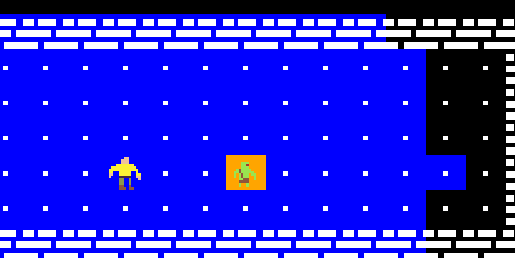
\includegraphics[width=8cm]{images/mygame/targeting.png}
	\caption{Wybór celu magicznego zwoju}
	\label{mygame:targeting}
\end{figure}
\FloatBarrier

\FloatBarrier
\begin{figure}[h]
	\centering
	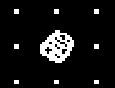
\includegraphics[width=3cm]{images/mygame/scroll.png}
	\caption{Magiczny zwój w grze}
	\label{mygame:scroll}
\end{figure}
\FloatBarrier

Dostępne w grze zwoje to 
\begin{itemize}
	\item 'Magic missile scroll' -- zwój magicznego pocisku, zadaje obrażenia wybranemu celowi,
	\item 'Fireball scroll' -- zwój ognistej kuli, zadaje obrażenia przeciwnikom w małym promieniu od wybranego celu,			
	\item 'Sleep scroll' -- zwój uśpienia, usypia wybrany cel na kilka tur -- nie będzie się on poruszał ani atakował,
	\item 'Area sleep scroll' -- zwój obszarowego uśpienia, usypia kilka przeciwników w małym promieniu od wybranego celu,
	\item 'Teleport scroll' -- zwój teleportacji, natychmiast przenosi postać gracza w wybrane miejsce.	
\end{itemize}


\subsection{Tester proceduralnie generowanych poziomów}
Gry roguelike opierają się w głównej mierze na proceduralnie generowanych poziomach, co oznacza generowanie map na podstawie algorytmów zawierających elementy losowości. Oznacza to na przykład, że użyty w niniejszej grze algorytm do generowania jaskiń zawsze wygeneruje poziom przypominający jaskinię, lecz za każdym razem inaczej wyglądający. Takie podejście do tworzenie poziomów pozwala znacznie zaosczędzić czas, który w standardowej metodzie byłby spędzony na ręcznie tworzenie poziomów. Mapy proceduralnie generowane są jednak podatne na błędy -- na przykład miejsca, do których nie da się dojść. W celu szybszego odnajdywania i naprawiania takich i podobnych błędów, a także w celu prezentacji możliwości zaimplementowanych algorytmów stworzono menu do testowania generatorów map, zaprezentowane na rysunku \ref{mygame:gen_test}. Menu to dostępne jest w głównym menu gry po wybraniu opcji 'Test Map Generators'.

\FloatBarrier
\begin{figure}[h]
	\centering
	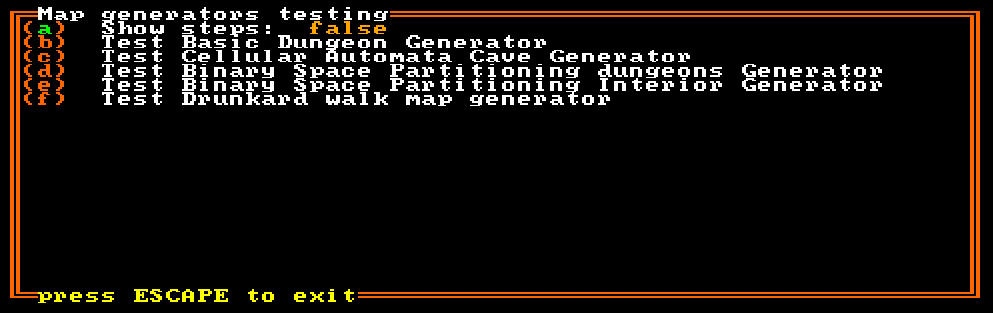
\includegraphics[width=14cm]{images/mygame/gen_test.png}
	\caption{Menu testera proceduralnie generowanych map}
	\label{mygame:gen_test}
\end{figure}
\FloatBarrier

Klawiszami strzałek oraz klawiszem Enter wybiera się opcję, klawiszem Esc można powrócić do głównego menu gry. Opcje dostępne w menu to:

\begin{enumerate}[label=\alph*), leftmargin=1.25cm]
	\item 'Show steps' -- zmiana opcji pokazania kroków generacji w trakcie testowania generatorów. 'true' oznacza włączenie pokazu kroków, 'false' wyłączenie,
	\item 'Test Basic Dungeon Generator' -- testowanie generacji poziomu 1,			
	\item 'Test Cellular Automata Cave Generator' -- testowanie generacji poziomu 3,
	\item 'Test Binary Space Partitioning dungeons Generator' -- testowanie generacji poziomu 2.
	\item 'Test Binary Space Partitioning Interior Generator' -- testowanie generacji poziomu 5.
	\item 'Test Drunkard walk map generator' -- testowanie generacji poziomu 4.
\end{enumerate}

Po wybrania generatora map otwiera się okno zaprezentowane na rysunku \ref{mygame:window_tester}. W głównej części zaprezentowany jest aktualny stan mapy w przypadku pokazu z krokami, lub finalny efekt generacji planszy w przypadku wyłączenia kroków. W dolnej części okna znajdują się informacje o numerze aktualnego kroku, oraz jego opisie. Klawiszem Esc powrócić można do menu testera, klawiszem spacji generuje się nową mapę lub przechodzi do kolejnego kroku.

\FloatBarrier
\begin{figure}[h]
	\centering
	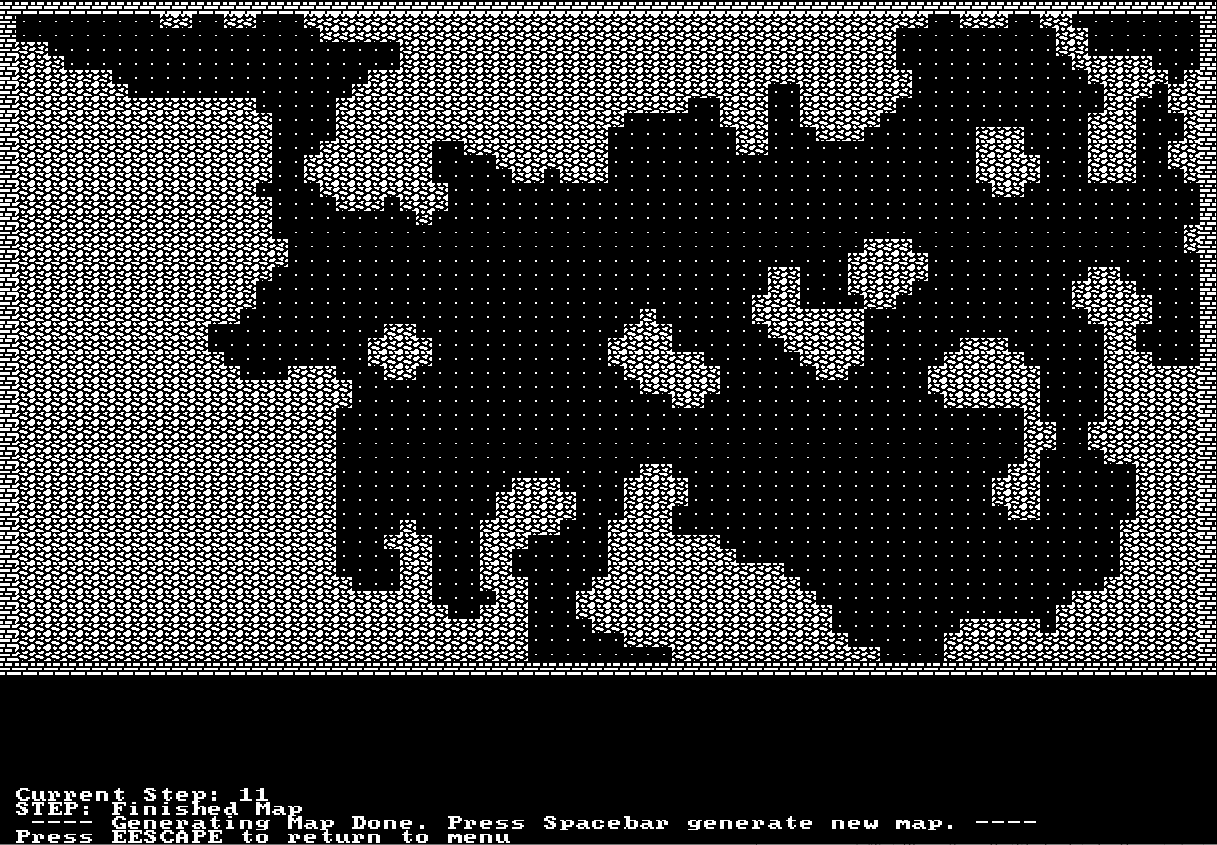
\includegraphics[width=14cm]{images/mygame/window_tester.png}
	\caption{Okno testera wybranego genratora map}
	\label{mygame:window_tester}
\end{figure}
\FloatBarrier

Na rysunku \ref{mygame:tester_steps} przedstawiono częśc kroków generacji mapy do poziomu trzeciego, na rysunku \ref{mygame:tester_nosteps} pokazano przykładowe wygenerowane mapy do poziomu drugiego.

\FloatBarrier
\begin{figure}[h]
	\centering
	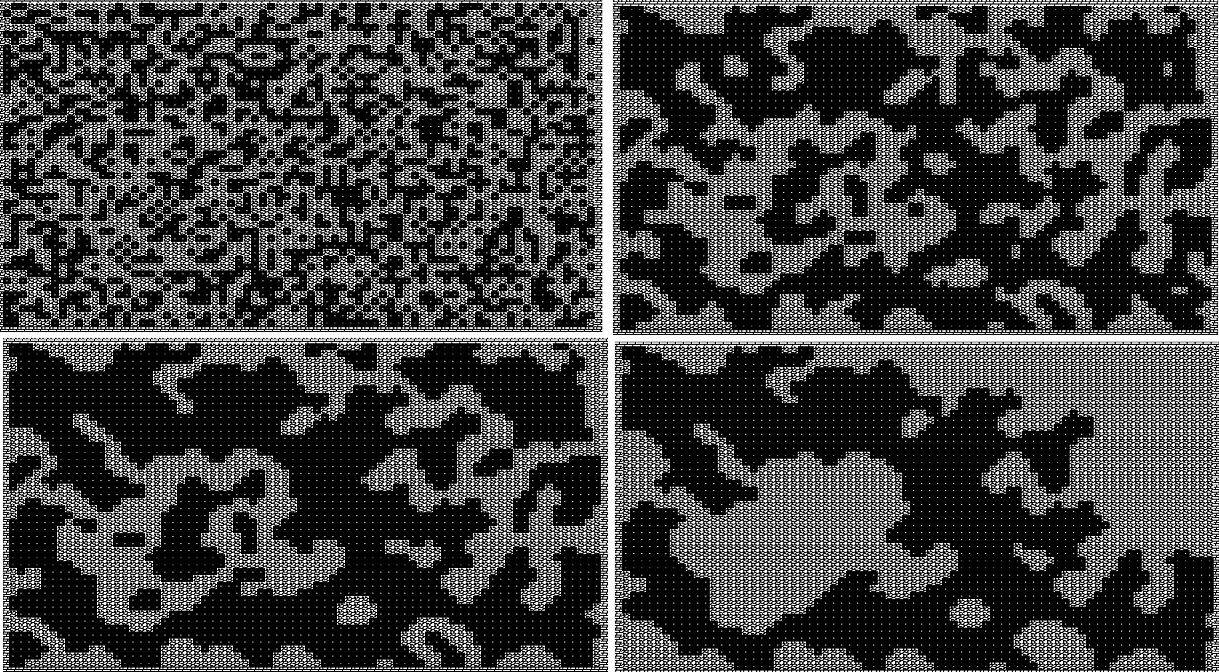
\includegraphics[width=16cm]{images/mygame/tester_steps.png}
	\caption{Przykład testowania z krokami generacji mapy do poziomu trzeciego}
	\label{mygame:tester_steps}
\end{figure}
\FloatBarrier

\FloatBarrier
\begin{figure}[h]
	\centering
	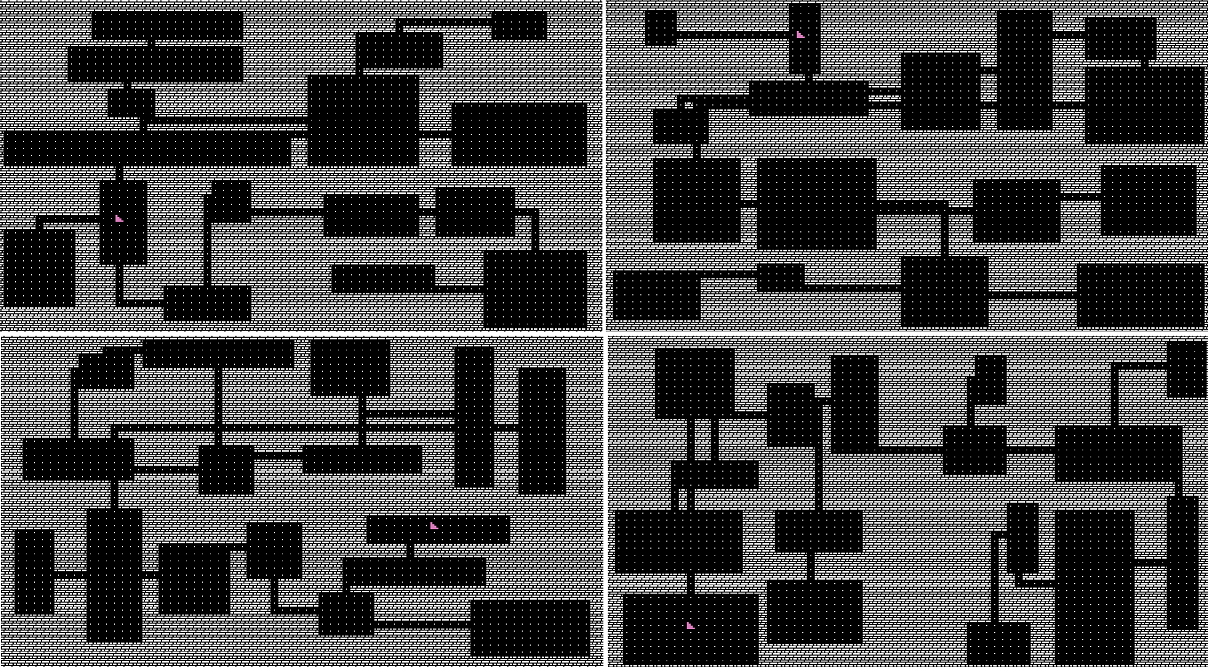
\includegraphics[width=16cm]{images/mygame/tester_nosteps.png}
	\caption{Przykład testowania bez kroków generacji mapy do poziomu drugiego}
	\label{mygame:tester_nosteps}
\end{figure}
\FloatBarrier

\clearpage	



\section{Technologie i implementacja}
W niniejszym rozdziale opisano technologie, architekturę oraz algorytmy użyte do implementacji gry.


\subsection{Technologie}
Do zaprogramowania gry użyto języka Rust, będącego kompilowalnym językiem ogólnego przeznaczenia, powstałym w 2010 roku \cite{book_rust}. Język Rust wydajnościowo jest porównywalny do języka C++, lecz jest to język nowocześniejszy i bezpieczniejszy \cite{rust_vs_cpp}. Język jest dużo bardziej restrykcyjny już na poziomie kompilacji, dzięki czemu błędy są częściej wykrywane w trakci kompilacji, niż dopiero po uruchomieniu programu. Użyto też wbudowanych w język narzędzi do formatowania 'cargo fmt' oraz lintera 'cargo clippy' -- który wykrywa niegroźne błędy nie wykrywane przez kompilator, ale utrudniające czytelność kodu. Te cechy oraz narzędzia języka Rust znacznie ułatwiają stosowanie zasad czystego kodu \cite{book_czystykod}.

Do edycji kodu użyty został program Visual Studio Code \cite{vs_code} z rozszerzeniami dla języka Rust, przede wszystkim 'rust-analyzer` zapewniający kolorowanie składni, oraz automatyczne uzupełnianie kodu.

W programie użyto wielu tworzonych przez społeczność bibliotek open source -- zapewniających prawo do korzystania, oraz dostęp do kodu źródłowego. Najważniejsze użyte biblioteki to:
\begin{itemize}
	\item `rltk` -- tworzenie okna gry, obsługa grafiki oraz pętli głównej gry,
	\item 'specs' -- implementacja architektury Entity Component System.
\end{itemize}

Gra posiada grafikę typu pixel art w formacie 16x16 pikseli, w oknie gry użyto dwukrotnie powięszonych obrazków w formacie 32x32 w celu polepszenia widoczności. Oryginalny format 16x16 używany jest w testerze proceduralnego generowania map w celu zaprezentowania całych map w jednym oknie. Do tworzenia grafiki użyto programu Aseprite \cite{aseprite} będącego wygodnym narzędziem graficznym wyspecjalizowanym w tworzeniu grafiki pixel art. Wszystkie obrazki użyte w grze znajdują się w folderze 'resources' w dwóch plikach, odpowiednio 'sprite\_sheet\_16x16.png' oraz 'sprite\_sheet\_32x32.png'. Taki format przechowywania obrazków zapewnia porządek w folderach gry, dostęp do konkretnego obrazka odbywa się przez określenie wymiarów oraz podaniu indeksu. Aby uzyskać obrazek przedstawiający gracza z pliku 'sprite\_sheet\_16x16.png' przedstawionego na rysunku \ref{mygame:spritesheet} należy określić rozmiary -- 16x16 pikseli oraz podać indeks 2 -- obrazki są indeksowane od lewej do prawej, pierwszy element ma indeks zero.

\FloatBarrier
\begin{figure}[h]
	\centering
	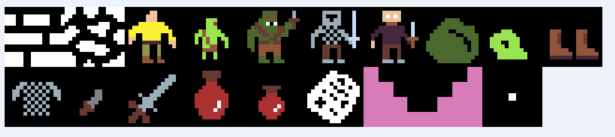
\includegraphics[width=12cm]{images/mygame/spritesheet.png}
	\caption{Grafiki użyte w grze}
	\label{mygame:spritesheet}
\end{figure}
\FloatBarrier















\iffalse


{\subsubsection{Listingi programów}}

W pracy dyplomowej możesz umieszczać fragmenty programów. Pamiętaj, aby umieszczać krótkie, tylko najważniejsze fragmenty kodów źródłowych. Zawsze je komentuj w treści
pracy dyplomowej. Typowo w \LaTeX\ kody źródłowe umieszczane są w środowisku verbatim (\verb|\begin{verbatim}...\end{verbatim}|). Obecnie instnieje jednak bardziej nowoczesne i bardziej funkcjonalne środowisko \verb|lstlisting| (wymaga zainstalowanego w systemie pakietu \verb|listings|). Zwróć uwagę, że możesz kolorować składnię
automatycznie za pomocą parametru \verb|language|. W niniejszym dokumencie przedstawiono dwa przykłady listingów, Listing \ref{KodMatlab1} to przykład kodu źródłowego Matlaba, a poniżej Listing \ref{KodPerl1} dla Perl'a.\\
%\komentarz{


% test listingu Rust - obrazki jednak beda lepsze
\begin{lstlisting}[language=Rust,caption=Listing programu Matlab,label={KodMatlab1}]
pub fn new(x: usize, y: usize, width: usize, height: usize) -> GuiMapGenTestingManager {
	GuiMapGenTestingManager {
		x,
		y,
		width,
		height,
		selected: 0,
		bg: rltk::RGB::named(rltk::BLACK),
		title: TextCol::new(vec![("Map generators testing".to_string(),rltk::RGB::named(rltk::WHITE))]),
		options: vec![],
		options_sprites_indexes: vec![],
		show_steps: false,
		map_gen: Box::new(TestMap::new(width - 4, height - 4)),
		current_history_index: 0,
	}
}
\end{lstlisting}

\begin{lstlisting}[language=Perl,caption=Listing programu Perl,label={KodPerl1}]
  my $url ='http://pei.prz.edu.pl';
  use LWP::Simple;
  my $content = get $url;
  die "Couldn't get $url" unless defined $content;
  print $content;
  print "\n";
  print "Length " + length($content)
\end{lstlisting}

Z pewnością przeglądając źródło tego dokumentu zobaczysz, że kody źródłowe powinny mieć zdefiniowane parametry \verb|label|, aby łatwo w tekście do nich się odwoływać.
Numeracja linii jest w stylu domyślnie włączona (to przydatne, bo w treści pracy łatwo odwołać się dzięki temu do konkretnego wiersza w kodzie źródłowym), możesz je wyłączyć podając jako parametr \verb|numbers=none|. Więcej szczegółów możesz odnaleźć w sekcji \verb|\lstset| pliku arkusza styli. 
%}


\subsubsection{Numerowanie i punktowanie}

\begin{enumerate}[label=\arabic*), leftmargin=1.25cm]
	\item Pierwszy poziom (stosuje się numerowanie lub punktowanie). Formatowanie:
	akapit wyjustowany, wcięcie od lewej 0,75 cm, wysunięcie co 0,5 cm.
	\item Znakiem numerowania jest liczba (z kropką lub nawiasem).
		\begin{itemize}[label=-,labelsep=0.4cm,leftmargin=0.6cm]
			\item drugi poziom (stosuje się wyłącznie punktowanie). Formatowanie: akapit
			wyjustowany, wcięcie od lewej 1,25 cm, wysunięcie co 0,5 cm,
			\item znakiem punktowania jest łącznik lub mała litera alfabetu (z nawiasem). Nie
			zaleca się stosowania kropek, strzałek itp.,
			\item punktowane akapity rozpoczyna się minuskułą (małą literą), na końcu akapitu
			stawia się przecinek, ostatni punktowany akapit kończy się kropką.
		\end{itemize}
	\item Numerowane akapity rozpoczyna się majuskułą (wielką literą) i kończy kropką.
	\item Należy zwrócić uwagę, aby nie rozdzielać numerowania/punktowania pomiędzy
	kolejnymi stronami tekstu.
\end{enumerate}


{\subsection{Wydruk pracy}}

Przed wydrukiem należy usunąć ewentualne błędy literowe i sprawdzić prawidłową
interpunkcję. Przykładowo, łącznik zapisuje się za pomocą krótkiego minusa (np.
badawczo-rozwojowy) natomiast myślnik -- stosowany w zdaniach wtrąconych -- zapisuje
się za pomocą długiej pauzy. Dzielenie wyrazów według uznania Autora (można podzielić
długie wyrazy, powodujące duże „rozstrzelenie” tekstu w poprzedzającym wierszu. Zaleca się usunięcie pojedynczych znaków na końcu wiersza oraz podwójnych spacji w tekście.
Dla przedrostka „mikro” należy unikać stosowania litery „u” zamiast „$\mu$”. Znak „$\mu$” można
otrzymać przytrzymując lewy Alt i wpisując na klawiaturze numerycznej 0181 (podobnie
„stopień”: Alt-0176). W celu uniknięcia „rozstrzelenia” liczb i ich jednostek zaleca się
używanie „twardej” spacji pomiędzy liczbą i jednostką. Należy sprawdzić, czy tytuły
podrozdziałów/zakresów nie zostały jako pojedyncze wiersze na poprzedniej stronie oraz
czy rysunki/tabele i ich tytuły nie zostały rozdzielone pomiędzy kolejnymi stronami.

Pracę drukuje się dwustronnie. Zaleca się wydruk w kolorze. Przed wydrukiem
należy ponumerować strony (czcionka 10 pkt., dół strony, akapit wyśrodkowany). Strony
tytułowej oraz strony z podziękowaniem nie numeruje się. Spis treści rozpoczyna się od
strony numer 3 (lub 5, jeżeli zamieszczono podziękowania).


\fi



\clearpage

\section{Podsumowanie i wnioski końcowe}


problemy i rozwiazania:
- mala widocznosc - powiekszono widok gry - przesuwajaca sie za graczm kamera


\clearpage

\section*{Załączniki}
\addcontentsline{toc}{section}{Załączniki}

Według potrzeb zawarte i uporządkowane uzupełnienie pracy o dowolny materiał źródłowy (wydruk programu komputerowego, dokumentacja kons\-truk\-cyj\-no-\-tech\-no\-lo\-gicz\-na, konstrukcja modelu -- makiety -- urządzenia, instrukcja obsługi urządzenia lub stanowiska laboratoryjnego, zestawienie wyników pomiarów i obliczeń, informacyjne materiały katalogowe itp.).


\clearpage

\addcontentsline{toc}{section}{Literatura}

\begin{thebibliography}{4}
	
% zrodlo film: Autor filmu [osoba/firma], tytuł, nazwa konferencji i odnośnik www.
% zrodlo gra : Autor gry [osoba/firma], nazwa gry i strona internetowa.

% ksiazka o komputerowych grach RPG
\bibitem{book_rpg} Felipe Pepe, The CRPG Book: A Guide to Computer Role-Playing Games, Bitmap Books, 2020.

% o roguelikach ogolnie https://www.routledge.com/Exploring-Roguelike-Games/Harris/p/book/9780367482596
\bibitem{bookroguelike} Harris J.: Exploring Roguelike Games. CRC Press, 2020.

% popularnosc nowoczesnych roguelike-ow
\bibitem{roguelike_popularity} Daniel Doan, Why Are Modern Roguelike Games So Popular?, https://gamedevlibrary.com/gamedev-thoughts-why-are-modern-roguelike-games-so-popular-53c1f5a05485.

% gra rogue (nie posiada oficjalnej strony)
\bibitem{rogue_game} Michael Toy, Glenn Wichman, Ken Arnold, Rogue, 1980, https://www.mobygames.com/game/rogue

% ksiazka o kodowaniu ascii
\bibitem{book_ascii} American Standards Association, American Standard Code for Information Interchange ASCII, 1963

% oficjalna strona gry caves of qud
\bibitem{game_coq} Freehold Games, Caves of Qud, 2015, https://www.cavesofqud.com

% artykul o pixel art
\bibitem{source_pixelart} Angie Kordic, What Exactly is Pixel Art and How Did It Come Back to Life ?, https://www.widewalls.ch/magazine/pixel-art

% oficjalna strona gry the binding of isaac
\bibitem{game_tboi} Edmund McMillen, Nicalis, The Binding of Isaac: Rebirth, 2014, https://bindingofisaac.com

% prezentacja o użyciu wave function collapse w Caves of Qud
\bibitem{coq_wfc} Brian Bucklew (Freehold Games), Math for Game Developers: Tile-Based Map Generation using Wave Function Collapse in 'Caves of Qud', Game Developers Conference, https://www.gdcvault.com/play/1026263/Math-for-Game-Developers-Tile .

% prezentacja o proceduralnej historii w Caves of Qud
\bibitem{coq_history} Jason Grinblat (Freehold Games), Procedurally Generating History in 'Caves of Qud', Game Developers Conference, https://www.gdcvault.com/play/1024990/Procedurally-Generating-History-in-Caves .

% Caves of qud w serwisie Steam
\bibitem{coq_steam} https://store.steampowered.com/app/333640/Caves\_of\_Qud/


%The binding of isaac w serwisie Steam
\bibitem{tboi_steam} https://store.steampowered.com/app/250900/The\_Binding\_of\_Isaac\_Rebirth/

% gra planszowa na podstawie tboi zebrala milion w tydzien
\bibitem{tboi_4souls} Stefanie Fogel, ‘The Binding of Isaac’ Card Game Surpasses 1 Million on Kickstarter in Just Over a Week, https://variety.com/2018/gaming/news/the-binding-of-isaac-four-souls-kickstarter-1202868455/


% ksiazka Rust
\bibitem{book_rust}  Steve Klabnik , Carol Nichols, The Rust Programming Language, No Starch Press, 2019.

% rust vs c++
\bibitem{rust_vs_cpp} Ben Fenwick, C++ v. Rust -Speed, Safety, \& Community Comparison, https://devetry.com/blog/c-v-rust-speed-safety-community-comparison/ .

% czysty kod
\bibitem{book_czystykod} Robert C. Martin, Czysty kod. Podręcznik dobrego programisty, Helion, 2014.

% vs code
\bibitem{vs_code} Microsoft, Visual Studio Code, 2015, https://code.visualstudio.com .

% program do pixel art
\bibitem{aseprite} Igara Studio S.A, Aseprite, 2001, https://www.aseprite.org.


% potencjalne zrodla:
% algorytmy i struktury danych



%notatki, pytania
\iffalse
czy dodac podrozdzial o przeciwnikach do opisu gry (okolo 1- 1.5 strony z obrazkami)
czy dodac zrodla o bibliotekach (2 strony github / crates.io)
czy w technologiach pisac o uzyciu gita i githuba + zrodlo github


\fi


\end{thebibliography}

\clearpage

\makesummary

\end{document} 
